\documentclass[twoside]{book}

% Packages required by doxygen
\usepackage{fixltx2e}
\usepackage{calc}
\usepackage{doxygen}
\usepackage[export]{adjustbox} % also loads graphicx
\usepackage{graphicx}
\usepackage[utf8]{inputenc}
\usepackage{makeidx}
\usepackage{multicol}
\usepackage{multirow}
\PassOptionsToPackage{warn}{textcomp}
\usepackage{textcomp}
\usepackage[nointegrals]{wasysym}
\usepackage[table]{xcolor}

% Font selection
\usepackage[T1]{fontenc}
\usepackage[scaled=.90]{helvet}
\usepackage{courier}
\usepackage{amssymb}
\usepackage{sectsty}
\renewcommand{\familydefault}{\sfdefault}
\allsectionsfont{%
  \fontseries{bc}\selectfont%
  \color{darkgray}%
}
\renewcommand{\DoxyLabelFont}{%
  \fontseries{bc}\selectfont%
  \color{darkgray}%
}
\newcommand{\+}{\discretionary{\mbox{\scriptsize$\hookleftarrow$}}{}{}}

% Page & text layout
\usepackage{geometry}
\geometry{%
  a4paper,%
  top=2.5cm,%
  bottom=2.5cm,%
  left=2.5cm,%
  right=2.5cm%
}
\tolerance=750
\hfuzz=15pt
\hbadness=750
\setlength{\emergencystretch}{15pt}
\setlength{\parindent}{0cm}
\setlength{\parskip}{3ex plus 2ex minus 2ex}
\makeatletter
\renewcommand{\paragraph}{%
  \@startsection{paragraph}{4}{0ex}{-1.0ex}{1.0ex}{%
    \normalfont\normalsize\bfseries\SS@parafont%
  }%
}
\renewcommand{\subparagraph}{%
  \@startsection{subparagraph}{5}{0ex}{-1.0ex}{1.0ex}{%
    \normalfont\normalsize\bfseries\SS@subparafont%
  }%
}
\makeatother

% Headers & footers
\usepackage{fancyhdr}
\pagestyle{fancyplain}
\fancyhead[LE]{\fancyplain{}{\bfseries\thepage}}
\fancyhead[CE]{\fancyplain{}{}}
\fancyhead[RE]{\fancyplain{}{\bfseries\leftmark}}
\fancyhead[LO]{\fancyplain{}{\bfseries\rightmark}}
\fancyhead[CO]{\fancyplain{}{}}
\fancyhead[RO]{\fancyplain{}{\bfseries\thepage}}
\fancyfoot[LE]{\fancyplain{}{}}
\fancyfoot[CE]{\fancyplain{}{}}
\fancyfoot[RE]{\fancyplain{}{\bfseries\scriptsize Generated by Doxygen }}
\fancyfoot[LO]{\fancyplain{}{\bfseries\scriptsize Generated by Doxygen }}
\fancyfoot[CO]{\fancyplain{}{}}
\fancyfoot[RO]{\fancyplain{}{}}
\renewcommand{\footrulewidth}{0.4pt}
\renewcommand{\chaptermark}[1]{%
  \markboth{#1}{}%
}
\renewcommand{\sectionmark}[1]{%
  \markright{\thesection\ #1}%
}

% Indices & bibliography
\usepackage{natbib}
\usepackage[titles]{tocloft}
\setcounter{tocdepth}{3}
\setcounter{secnumdepth}{5}
\makeindex

% Hyperlinks (required, but should be loaded last)
\usepackage{ifpdf}
\ifpdf
  \usepackage[pdftex,pagebackref=true]{hyperref}
\else
  \usepackage[ps2pdf,pagebackref=true]{hyperref}
\fi
\hypersetup{%
  colorlinks=true,%
  linkcolor=blue,%
  citecolor=blue,%
  unicode%
}

% Custom commands
\newcommand{\clearemptydoublepage}{%
  \newpage{\pagestyle{empty}\cleardoublepage}%
}

\usepackage{caption}
\captionsetup{labelsep=space,justification=centering,font={bf},singlelinecheck=off,skip=4pt,position=top}

%===== C O N T E N T S =====

\begin{document}

% Titlepage & ToC
\hypersetup{pageanchor=false,
             bookmarksnumbered=true,
             pdfencoding=unicode
            }
\pagenumbering{alph}
\begin{titlepage}
\vspace*{7cm}
\begin{center}%
{\Large Jet\+Pack\+Joy\+Ride }\\
\vspace*{1cm}
{\large Generated by Doxygen 1.8.13}\\
\end{center}
\end{titlepage}
\clearemptydoublepage
\pagenumbering{roman}
\tableofcontents
\clearemptydoublepage
\pagenumbering{arabic}
\hypersetup{pageanchor=true}

%--- Begin generated contents ---
\chapter{R\+O\+S2 Lane keeping workspace}
\label{index}\hypertarget{index}{}\subsection*{Overview}

This R\+O\+S2-\/based system runs on a Jetson Nano and processes camera input to detect lane markings and control vehicle motion accordingly. The system consists of multiple nodes that handle image capture, lane detection, motion control, and visualization.

\subsubsection*{High-\/\+Level System Flow\+:}


\begin{DoxyEnumerate}
\item {\bfseries Camera Node}\+: Captures and publishes raw image data.
\item {\bfseries Vision Processing Nodes}\+: Extract lane markings and publish lane position data.
\item {\bfseries Motion Control Node}\+: Estimates lane distance and adjusts steering.
\item {\bfseries Lane Visualization Node}\+: Publishes processed lane data for visualization in Rviz.
\end{DoxyEnumerate}

\subsection*{Software architecture}



\subsection*{Node Descriptions}

\subsubsection*{1. Camera Node ({\ttfamily camera})}

{\bfseries Function}\+: Captures image frames and publishes them.
\begin{DoxyItemize}
\item {\bfseries Publishes}\+:
\begin{DoxyItemize}
\item {\ttfamily /image\+\_\+raw} (sensor\+\_\+msgs\+::\+Image)
\end{DoxyItemize}
\end{DoxyItemize}

\subsubsection*{2. Classic Vision Node ({\ttfamily classic\+\_\+vision})}

{\bfseries Function}\+: Processes raw images to detect lane markings using Open\+CV.
\begin{DoxyItemize}
\item {\bfseries Subscribes}\+:
\begin{DoxyItemize}
\item {\ttfamily /image\+\_\+raw} (sensor\+\_\+msgs\+::\+Image)
\end{DoxyItemize}
\item {\bfseries Publishes}\+:
\begin{DoxyItemize}
\item {\ttfamily /lane\+\_\+position} (custom message)
\end{DoxyItemize}
\item {\bfseries Parameters}\+:
\begin{DoxyItemize}
\item {\ttfamily low\+\_\+canny\+\_\+threshold} / {\ttfamily high\+\_\+canny\+\_\+treshold}\+: Edge detection parameters
\item {\ttfamily hough\+\_\+transform\+\_\+params}\+: Line detection parameters
\begin{DoxyItemize}
\item {\ttfamily max\+\_\+detected\+\_\+lines}
\item {\ttfamily max\+\_\+line\+\_\+gap}
\item {\ttfamily mine\+\_\+line\+\_\+length}
\item {\ttfamily rho}
\end{DoxyItemize}
\end{DoxyItemize}
\end{DoxyItemize}

\subsubsection*{3. Classic Vision Node ({\ttfamily classic\+\_\+vision})}

{\bfseries Function}\+: Processes raw images to detect lane markings using Tensor\+RT.
\begin{DoxyItemize}
\item {\bfseries Subscribes}\+:
\begin{DoxyItemize}
\item {\ttfamily /image\+\_\+raw} (sensor\+\_\+msgs\+::\+Image)
\end{DoxyItemize}
\item {\bfseries Publishes}\+:
\begin{DoxyItemize}
\item {\ttfamily /lane\+\_\+position} (custom message)
\end{DoxyItemize}
\end{DoxyItemize}

\subsubsection*{4. Image Publisher Node ({\ttfamily image\+\_\+publisher})}

{\bfseries Function}\+: Auxiliary node for testing image data flow.
\begin{DoxyItemize}
\item {\bfseries Publishes}\+:
\begin{DoxyItemize}
\item {\ttfamily /debug\+\_\+image} (sensor\+\_\+msgs\+::\+Image)
\end{DoxyItemize}
\item {\bfseries Parameters}\+:
\begin{DoxyItemize}
\item {\ttfamily image\+\_\+name}\+: image from assets folder
\end{DoxyItemize}
\end{DoxyItemize}

\subsubsection*{5. Lane Messages ({\ttfamily lane\+\_\+msgs})}

{\bfseries Function}\+: Defines custom message types for lane detection data.
\begin{DoxyItemize}
\item {\bfseries Custom Messages}\+:
\begin{DoxyItemize}
\item {\ttfamily Lane\+Position.\+msg}\+: Lane position relative to vehicle
\end{DoxyItemize}
\end{DoxyItemize}

\subsubsection*{6. Lane Visualization ({\ttfamily lane\+\_\+visualization})}

{\bfseries Function}\+: Publishes visual representation of lane\+\_\+position.
\begin{DoxyItemize}
\item {\bfseries Subscribes}\+:
\begin{DoxyItemize}
\item {\ttfamily /lane\+\_\+position} (custom message)
\end{DoxyItemize}
\item {\bfseries Publishes}\+:
\begin{DoxyItemize}
\item {\ttfamily /processed\+\_\+img} (sensor\+\_\+msgs\+::\+Image)
\end{DoxyItemize}
\end{DoxyItemize}

\subsubsection*{7. Motion Control Node ({\ttfamily motion\+\_\+control})}

{\bfseries Function}\+: Computes steering commands based on lane position.
\begin{DoxyItemize}
\item {\bfseries Subscribes}\+:
\begin{DoxyItemize}
\item {\ttfamily /lane\+\_\+position} (custom message)
\end{DoxyItemize}
\item {\bfseries Publishes}\+:
\begin{DoxyItemize}
\item {\ttfamily /cmd\+\_\+vel} (geometry\+\_\+msgs\+::\+Twist)
\end{DoxyItemize}
\item {\bfseries Parameters}\+:
\begin{DoxyItemize}
\item {\ttfamily base\+\_\+speed}\+: base speed of vehicle
\item {\ttfamily lookahead\+\_\+index}\+: distance (in buckets) to the reference point
\item {\ttfamily kp}, {\ttfamily ki}, {\ttfamily kd}\+: proportional, integral and derivative gain. 
\end{DoxyItemize}
\end{DoxyItemize}
\chapter{Hierarchical Index}
\section{Class Hierarchy}
This inheritance list is sorted roughly, but not completely, alphabetically\+:\begin{DoxyCompactList}
\item \contentsline{section}{cuda\+Deleter$<$ T $>$}{\pageref{structcudaDeleter}}{}
\item I\+Logger\begin{DoxyCompactList}
\item \contentsline{section}{Logger}{\pageref{classLogger}}{}
\end{DoxyCompactList}
\item \contentsline{section}{Image\+Processor}{\pageref{classImageProcessor}}{}
\item \contentsline{section}{Inference\+Engine}{\pageref{classInferenceEngine}}{}
\item \contentsline{section}{Kalman\+Filter}{\pageref{classKalmanFilter}}{}
\item \contentsline{section}{Lane\+Buffer}{\pageref{classLaneBuffer}}{}
\item Node\begin{DoxyCompactList}
\item \contentsline{section}{Camera\+Node}{\pageref{classCameraNode}}{}
\item \contentsline{section}{Image\+Publisher\+Node}{\pageref{classImagePublisherNode}}{}
\item \contentsline{section}{Lane\+Visualization\+Node}{\pageref{classLaneVisualizationNode}}{}
\item \contentsline{section}{Ml\+Vision\+Node}{\pageref{classMlVisionNode}}{}
\item \contentsline{section}{Motion\+Control\+Node}{\pageref{classMotionControlNode}}{}
\item \contentsline{section}{Vision\+Node}{\pageref{classVisionNode}}{}
\end{DoxyCompactList}
\item \contentsline{section}{P\+I\+D\+Controller}{\pageref{classPIDController}}{}
\item Test\begin{DoxyCompactList}
\item \contentsline{section}{Lane\+Buffer\+Test}{\pageref{classLaneBufferTest}}{}
\end{DoxyCompactList}
\item \contentsline{section}{Trt\+Deleter$<$ T $>$}{\pageref{structTrtDeleter}}{}
\end{DoxyCompactList}

\chapter{Class Index}
\section{Class List}
Here are the classes, structs, unions and interfaces with brief descriptions\+:\begin{DoxyCompactList}
\item\contentsline{section}{\hyperlink{classCameraNode}{Camera\+Node} \\*Captures and publish camera frames using Open\+CV with G\+Streamer }{\pageref{classCameraNode}}{}
\item\contentsline{section}{\hyperlink{structcudaDeleter}{cuda\+Deleter$<$ T $>$} \\*Custom deleter for Cuda allocations }{\pageref{structcudaDeleter}}{}
\item\contentsline{section}{\hyperlink{classImageProcessor}{Image\+Processor} \\*Handles image preprocessing and feature extraction on the G\+PU using Open\+CV C\+U\+DA }{\pageref{classImageProcessor}}{}
\item\contentsline{section}{\hyperlink{classImagePublisherNode}{Image\+Publisher\+Node} }{\pageref{classImagePublisherNode}}{}
\item\contentsline{section}{\hyperlink{classInferenceEngine}{Inference\+Engine} \\*Encapsulates Tensor\+RT engine creation, memory management, and inference execution }{\pageref{classInferenceEngine}}{}
\item\contentsline{section}{\hyperlink{classKalmanFilter}{Kalman\+Filter} \\*1d Kalman filter }{\pageref{classKalmanFilter}}{}
\item\contentsline{section}{\hyperlink{classLaneBuffer}{Lane\+Buffer} }{\pageref{classLaneBuffer}}{}
\item\contentsline{section}{\hyperlink{classLaneBufferTest}{Lane\+Buffer\+Test} }{\pageref{classLaneBufferTest}}{}
\item\contentsline{section}{\hyperlink{classLaneVisualizationNode}{Lane\+Visualization\+Node} \\*Display the geometries published by the vision and motion node (lane positions, polyfits...) }{\pageref{classLaneVisualizationNode}}{}
\item\contentsline{section}{\hyperlink{classLogger}{Logger} }{\pageref{classLogger}}{}
\item\contentsline{section}{\hyperlink{classMlVisionNode}{Ml\+Vision\+Node} \\*Performs lane detection using a deep learning model accelerated with Tensor\+RT and C\+U\+D\+A-\/based image preprocessing }{\pageref{classMlVisionNode}}{}
\item\contentsline{section}{\hyperlink{classMotionControlNode}{Motion\+Control\+Node} \\*Implements lane-\/keeping control using polynomial fitting and P\+ID control }{\pageref{classMotionControlNode}}{}
\item\contentsline{section}{\hyperlink{classPIDController}{P\+I\+D\+Controller} }{\pageref{classPIDController}}{}
\item\contentsline{section}{\hyperlink{structTrtDeleter}{Trt\+Deleter$<$ T $>$} \\*Custom deleter for T\+RT objects }{\pageref{structTrtDeleter}}{}
\item\contentsline{section}{\hyperlink{classVisionNode}{Vision\+Node} \\*Processes camera images to detect lane positions using G\+P\+U-\/accelerated Open\+CV }{\pageref{classVisionNode}}{}
\end{DoxyCompactList}

\chapter{Class Documentation}
\hypertarget{classCameraNode}{}\section{Camera\+Node Class Reference}
\label{classCameraNode}\index{Camera\+Node@{Camera\+Node}}


Captures and publish camera frames using Open\+CV with G\+Streamer.  




{\ttfamily \#include $<$Camera\+Node.\+hpp$>$}



Inheritance diagram for Camera\+Node\+:
\nopagebreak
\begin{figure}[H]
\begin{center}
\leavevmode
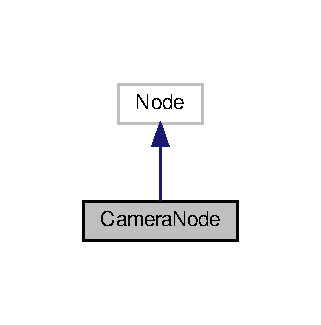
\includegraphics[width=154pt]{classCameraNode__inherit__graph}
\end{center}
\end{figure}


Collaboration diagram for Camera\+Node\+:
\nopagebreak
\begin{figure}[H]
\begin{center}
\leavevmode
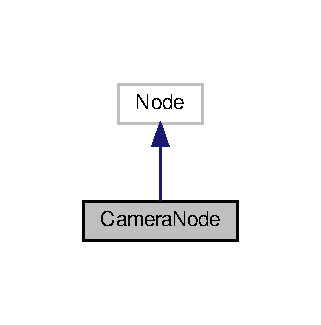
\includegraphics[width=154pt]{classCameraNode__coll__graph}
\end{center}
\end{figure}
\subsection*{Public Member Functions}
\begin{DoxyCompactItemize}
\item 
\hyperlink{classCameraNode_ab3a466dc9357b5200fb6843a6d64c5c8}{$\sim$\+Camera\+Node} ()
\begin{DoxyCompactList}\small\item\em Ensures safe shutdown of the \hyperlink{classCameraNode}{Camera\+Node}. \end{DoxyCompactList}\end{DoxyCompactItemize}
\subsection*{Private Member Functions}
\begin{DoxyCompactItemize}
\item 
void \hyperlink{classCameraNode_ae82e95951417f976eed687ddf64c6d9f}{init\+Publisher\+And\+Capture} ()
\begin{DoxyCompactList}\small\item\em Initializes the R\+O\+S2 image publisher and starts frame capture. \end{DoxyCompactList}\item 
void \hyperlink{classCameraNode_a1a44c8d8757a75cf649cbcf49cfa1ca1}{capture\+Frame} ()
\begin{DoxyCompactList}\small\item\em Continuously captures frames and publishes them to R\+O\+S2. \end{DoxyCompactList}\end{DoxyCompactItemize}
\subsection*{Private Attributes}
\begin{DoxyCompactItemize}
\item 
\mbox{\Hypertarget{classCameraNode_a589ef67a59d2205bb65beeaef950fb29}\label{classCameraNode_a589ef67a59d2205bb65beeaef950fb29}} 
std\+::atomic$<$ bool $>$ {\bfseries running\+\_\+}
\item 
\mbox{\Hypertarget{classCameraNode_ad29d310c3d87b40124d35562c62af9ef}\label{classCameraNode_ad29d310c3d87b40124d35562c62af9ef}} 
std\+::thread {\bfseries capture\+\_\+thread\+\_\+}
\item 
\mbox{\Hypertarget{classCameraNode_a4d4f490deef80022a254d3de565f2611}\label{classCameraNode_a4d4f490deef80022a254d3de565f2611}} 
cv\+::\+Video\+Capture {\bfseries cap\+\_\+}
\item 
\mbox{\Hypertarget{classCameraNode_a59ce8fd47a93d1baecb2611ee5336d7b}\label{classCameraNode_a59ce8fd47a93d1baecb2611ee5336d7b}} 
image\+\_\+transport\+::\+Publisher {\bfseries image\+\_\+pub\+\_\+}
\end{DoxyCompactItemize}


\subsection{Detailed Description}
Captures and publish camera frames using Open\+CV with G\+Streamer. 

This node initializes a camera pipeline (using nvidia camera stack and gstreamer), captures frames in a dedicated thread, and publishes them as R\+O\+S2 sensor\+\_\+msgs/\+Image messages on the \char`\"{}image\+\_\+raw\char`\"{} topic. 

\subsection{Constructor \& Destructor Documentation}
\mbox{\Hypertarget{classCameraNode_ab3a466dc9357b5200fb6843a6d64c5c8}\label{classCameraNode_ab3a466dc9357b5200fb6843a6d64c5c8}} 
\index{Camera\+Node@{Camera\+Node}!````~Camera\+Node@{$\sim$\+Camera\+Node}}
\index{````~Camera\+Node@{$\sim$\+Camera\+Node}!Camera\+Node@{Camera\+Node}}
\subsubsection{\texorpdfstring{$\sim$\+Camera\+Node()}{~CameraNode()}}
{\footnotesize\ttfamily Camera\+Node\+::$\sim$\+Camera\+Node (\begin{DoxyParamCaption}{ }\end{DoxyParamCaption})}



Ensures safe shutdown of the \hyperlink{classCameraNode}{Camera\+Node}. 


\begin{DoxyItemize}
\item Signals the capture thread to stop ({\ttfamily running\+\_\+ = false}).
\item Joins the thread if it\textquotesingle{}s still running.
\item Releases the Open\+CV camera resource. 
\end{DoxyItemize}

\subsection{Member Function Documentation}
\mbox{\Hypertarget{classCameraNode_a1a44c8d8757a75cf649cbcf49cfa1ca1}\label{classCameraNode_a1a44c8d8757a75cf649cbcf49cfa1ca1}} 
\index{Camera\+Node@{Camera\+Node}!capture\+Frame@{capture\+Frame}}
\index{capture\+Frame@{capture\+Frame}!Camera\+Node@{Camera\+Node}}
\subsubsection{\texorpdfstring{capture\+Frame()}{captureFrame()}}
{\footnotesize\ttfamily void Camera\+Node\+::capture\+Frame (\begin{DoxyParamCaption}{ }\end{DoxyParamCaption})\hspace{0.3cm}{\ttfamily [private]}}



Continuously captures frames and publishes them to R\+O\+S2. 


\begin{DoxyItemize}
\item Reads frames from the camera in a loop (non-\/blocking).
\item Converts each Open\+CV {\ttfamily Mat} frame to a R\+O\+S2 {\ttfamily sensor\+\_\+msgs/\+Image}.
\item Publishes the image message on the \char`\"{}image\+\_\+raw\char`\"{} topic.
\item Exits gracefully if R\+O\+S2 is shutdown ({\ttfamily rclcpp\+::ok()}) or an error occurs. 
\end{DoxyItemize}\mbox{\Hypertarget{classCameraNode_ae82e95951417f976eed687ddf64c6d9f}\label{classCameraNode_ae82e95951417f976eed687ddf64c6d9f}} 
\index{Camera\+Node@{Camera\+Node}!init\+Publisher\+And\+Capture@{init\+Publisher\+And\+Capture}}
\index{init\+Publisher\+And\+Capture@{init\+Publisher\+And\+Capture}!Camera\+Node@{Camera\+Node}}
\subsubsection{\texorpdfstring{init\+Publisher\+And\+Capture()}{initPublisherAndCapture()}}
{\footnotesize\ttfamily void Camera\+Node\+::init\+Publisher\+And\+Capture (\begin{DoxyParamCaption}{ }\end{DoxyParamCaption})\hspace{0.3cm}{\ttfamily [private]}}



Initializes the R\+O\+S2 image publisher and starts frame capture. 


\begin{DoxyItemize}
\item Creates an {\ttfamily image\+\_\+transport\+::\+Image\+Transport} for efficient image publishing.
\item Advertises the \char`\"{}image\+\_\+raw\char`\"{} topic.
\item Calls {\ttfamily \hyperlink{classCameraNode_a1a44c8d8757a75cf649cbcf49cfa1ca1}{capture\+Frame()}} to begin the capture loop. 
\end{DoxyItemize}

The documentation for this class was generated from the following files\+:\begin{DoxyCompactItemize}
\item 
lane\+\_\+keeping\+\_\+ws/src/camera/includes/Camera\+Node.\+hpp\item 
lane\+\_\+keeping\+\_\+ws/src/camera/src/Camera\+Node.\+cpp\end{DoxyCompactItemize}

\hypertarget{structcudaDeleter}{}\section{cuda\+Deleter$<$ T $>$ Struct Template Reference}
\label{structcudaDeleter}\index{cuda\+Deleter$<$ T $>$@{cuda\+Deleter$<$ T $>$}}


custom deleter for Cuda allocations  




{\ttfamily \#include $<$Inference\+Engine.\+hpp$>$}

\subsection*{Public Member Functions}
\begin{DoxyCompactItemize}
\item 
\mbox{\Hypertarget{structcudaDeleter_abb2b0fa5a5f7ddcd45a9b8ce2cdf1f28}\label{structcudaDeleter_abb2b0fa5a5f7ddcd45a9b8ce2cdf1f28}} 
void {\bfseries operator()} (T $\ast$ptr) const
\end{DoxyCompactItemize}


\subsection{Detailed Description}
\subsubsection*{template$<$typename T$>$\newline
struct cuda\+Deleter$<$ T $>$}

custom deleter for Cuda allocations 


\begin{DoxyTemplParams}{Template Parameters}
{\em T} & \\
\hline
\end{DoxyTemplParams}

\begin{DoxyParams}{Parameters}
{\em ptr} & \\
\hline
\end{DoxyParams}


The documentation for this struct was generated from the following file\+:\begin{DoxyCompactItemize}
\item 
lane\+\_\+keeping\+\_\+ws/src/ml\+\_\+vision/includes/Inference\+Engine.\+hpp\end{DoxyCompactItemize}

\hypertarget{classImageProcessor}{}\section{Image\+Processor Class Reference}
\label{classImageProcessor}\index{Image\+Processor@{Image\+Processor}}


Handles image preprocessing and feature extraction on the G\+PU using Open\+CV C\+U\+DA.  




{\ttfamily \#include $<$Image\+Processor.\+hpp$>$}

\subsection*{Public Member Functions}
\begin{DoxyCompactItemize}
\item 
\hyperlink{classImageProcessor_af52cf1abf1dacffda01cc55b6f5c8313}{Image\+Processor} (const cv\+::\+Size \&input\+\_\+size, const cv\+::\+Size \&output\+\_\+size)
\begin{DoxyCompactList}\small\item\em Construct a new \hyperlink{classImageProcessor}{Image\+Processor} object. \end{DoxyCompactList}\item 
std\+::vector$<$ float $>$ \hyperlink{classImageProcessor_a9e6ce929aa19b3dc53d855ce0f68a2f6}{flatten\+Image} (cv\+::\+Mat \&img) const
\begin{DoxyCompactList}\small\item\em Resizes and normalizes a B\+GR image, flattening it into a float vector. \end{DoxyCompactList}\item 
void \hyperlink{classImageProcessor_a6bce7d61162f71ae9bb322b40c9990ab}{apply\+Treshold} (cv\+::cuda\+::\+Gpu\+Mat \&gpu\+\_\+img, int treshold)
\begin{DoxyCompactList}\small\item\em Applies a binary threshold on a G\+PU image. \end{DoxyCompactList}\item 
void \hyperlink{classImageProcessor_a358c5380af94e810845282f05579265a}{apply\+Erosion\+Dilation} (cv\+::cuda\+::\+Gpu\+Mat \&gpu\+\_\+img)
\begin{DoxyCompactList}\small\item\em Applies dilation followed by erosion (closing) to reduce noise. \end{DoxyCompactList}\item 
void \hyperlink{classImageProcessor_a54826c571dfde1f85fec2ad86f21f69a}{apply\+Canny\+Edge} (cv\+::cuda\+::\+Gpu\+Mat \&gpu\+\_\+img)
\begin{DoxyCompactList}\small\item\em Applies the Canny edge detector to a G\+PU image. \end{DoxyCompactList}\item 
std\+::vector$<$ cv\+::\+Vec4i $>$ \hyperlink{classImageProcessor_aaceb6004986b3c9c61084531dbb12011}{get\+Lines} (cv\+::cuda\+::\+Gpu\+Mat \&gpu\+\_\+img)
\begin{DoxyCompactList}\small\item\em Extracts lines from an edge-\/detected image using Hough Transform. \end{DoxyCompactList}\end{DoxyCompactItemize}
\subsection*{Private Attributes}
\begin{DoxyCompactItemize}
\item 
\mbox{\Hypertarget{classImageProcessor_a964238c103b14e74afab0ebc9671bc88}\label{classImageProcessor_a964238c103b14e74afab0ebc9671bc88}} 
cv\+::\+Size {\bfseries input\+\_\+size\+\_\+}
\item 
\mbox{\Hypertarget{classImageProcessor_a8686621bd8c62a575c221ae45f9e70b9}\label{classImageProcessor_a8686621bd8c62a575c221ae45f9e70b9}} 
cv\+::\+Size {\bfseries output\+\_\+size\+\_\+}
\item 
\mbox{\Hypertarget{classImageProcessor_a873e79e99bc7c9f7602fde8d8e47aa76}\label{classImageProcessor_a873e79e99bc7c9f7602fde8d8e47aa76}} 
cv\+::\+Ptr$<$ cv\+::cuda\+::\+Canny\+Edge\+Detector $>$ {\bfseries canny\+\_\+edge\+\_\+detector\+\_\+}
\item 
\mbox{\Hypertarget{classImageProcessor_a56f6caa5183f0f2000a094fcf2cdf1a5}\label{classImageProcessor_a56f6caa5183f0f2000a094fcf2cdf1a5}} 
cv\+::\+Ptr$<$ cv\+::cuda\+::\+Hough\+Segment\+Detector $>$ {\bfseries line\+\_\+detector\+\_\+}
\item 
\mbox{\Hypertarget{classImageProcessor_a9e2ba2ac27b9c0d5b38e05ccc52d67ca}\label{classImageProcessor_a9e2ba2ac27b9c0d5b38e05ccc52d67ca}} 
cv\+::\+Ptr$<$ cv\+::cuda\+::\+Filter $>$ {\bfseries erosion\+\_\+filter\+\_\+}
\item 
\mbox{\Hypertarget{classImageProcessor_a46acab87bda21888d9cec25857661aff}\label{classImageProcessor_a46acab87bda21888d9cec25857661aff}} 
cv\+::\+Ptr$<$ cv\+::cuda\+::\+Filter $>$ {\bfseries dilation\+\_\+filter\+\_\+}
\end{DoxyCompactItemize}


\subsection{Detailed Description}
Handles image preprocessing and feature extraction on the G\+PU using Open\+CV C\+U\+DA. 

This class provides functionality for preparing images for machine learning inference, including resizing, flattening, edge detection, thresholding, morphological operations, and line detection via Hough Transform. 

\subsection{Constructor \& Destructor Documentation}
\mbox{\Hypertarget{classImageProcessor_af52cf1abf1dacffda01cc55b6f5c8313}\label{classImageProcessor_af52cf1abf1dacffda01cc55b6f5c8313}} 
\index{Image\+Processor@{Image\+Processor}!Image\+Processor@{Image\+Processor}}
\index{Image\+Processor@{Image\+Processor}!Image\+Processor@{Image\+Processor}}
\subsubsection{\texorpdfstring{Image\+Processor()}{ImageProcessor()}}
{\footnotesize\ttfamily Image\+Processor\+::\+Image\+Processor (\begin{DoxyParamCaption}\item[{const cv\+::\+Size \&}]{input\+\_\+size,  }\item[{const cv\+::\+Size \&}]{output\+\_\+size }\end{DoxyParamCaption})}



Construct a new \hyperlink{classImageProcessor}{Image\+Processor} object. 

Initializes all C\+U\+DA filters and detectors using the given input and output sizes.


\begin{DoxyParams}{Parameters}
{\em input\+\_\+size} & Expected input size for the ML model. \\
\hline
{\em output\+\_\+size} & Expected size for post-\/processed output (if needed). \\
\hline
\end{DoxyParams}


\subsection{Member Function Documentation}
\mbox{\Hypertarget{classImageProcessor_a54826c571dfde1f85fec2ad86f21f69a}\label{classImageProcessor_a54826c571dfde1f85fec2ad86f21f69a}} 
\index{Image\+Processor@{Image\+Processor}!apply\+Canny\+Edge@{apply\+Canny\+Edge}}
\index{apply\+Canny\+Edge@{apply\+Canny\+Edge}!Image\+Processor@{Image\+Processor}}
\subsubsection{\texorpdfstring{apply\+Canny\+Edge()}{applyCannyEdge()}}
{\footnotesize\ttfamily void Image\+Processor\+::apply\+Canny\+Edge (\begin{DoxyParamCaption}\item[{cv\+::cuda\+::\+Gpu\+Mat \&}]{gpu\+\_\+img }\end{DoxyParamCaption})}



Applies the Canny edge detector to a G\+PU image. 

Detects edges in the image using C\+U\+D\+A-\/accelerated Canny filter.


\begin{DoxyParams}{Parameters}
{\em gpu\+\_\+img} & Image on which to apply edge detection (in-\/place). \\
\hline
\end{DoxyParams}
\mbox{\Hypertarget{classImageProcessor_a358c5380af94e810845282f05579265a}\label{classImageProcessor_a358c5380af94e810845282f05579265a}} 
\index{Image\+Processor@{Image\+Processor}!apply\+Erosion\+Dilation@{apply\+Erosion\+Dilation}}
\index{apply\+Erosion\+Dilation@{apply\+Erosion\+Dilation}!Image\+Processor@{Image\+Processor}}
\subsubsection{\texorpdfstring{apply\+Erosion\+Dilation()}{applyErosionDilation()}}
{\footnotesize\ttfamily void Image\+Processor\+::apply\+Erosion\+Dilation (\begin{DoxyParamCaption}\item[{cv\+::cuda\+::\+Gpu\+Mat \&}]{gpu\+\_\+img }\end{DoxyParamCaption})}



Applies dilation followed by erosion (closing) to reduce noise. 

This is useful for filling small gaps in detected edges or lines.


\begin{DoxyParams}{Parameters}
{\em gpu\+\_\+img} & Image on which to apply morphological operations (in-\/place). \\
\hline
\end{DoxyParams}
\mbox{\Hypertarget{classImageProcessor_a6bce7d61162f71ae9bb322b40c9990ab}\label{classImageProcessor_a6bce7d61162f71ae9bb322b40c9990ab}} 
\index{Image\+Processor@{Image\+Processor}!apply\+Treshold@{apply\+Treshold}}
\index{apply\+Treshold@{apply\+Treshold}!Image\+Processor@{Image\+Processor}}
\subsubsection{\texorpdfstring{apply\+Treshold()}{applyTreshold()}}
{\footnotesize\ttfamily void Image\+Processor\+::apply\+Treshold (\begin{DoxyParamCaption}\item[{cv\+::cuda\+::\+Gpu\+Mat \&}]{gpu\+\_\+img,  }\item[{int}]{treshold }\end{DoxyParamCaption})}



Applies a binary threshold on a G\+PU image. 

All values above the threshold are set to 255; others are set to 0.


\begin{DoxyParams}{Parameters}
{\em gpu\+\_\+img} & Image on which to apply thresholding (in-\/place). \\
\hline
{\em treshold} & Threshold value. \\
\hline
\end{DoxyParams}
\mbox{\Hypertarget{classImageProcessor_a9e6ce929aa19b3dc53d855ce0f68a2f6}\label{classImageProcessor_a9e6ce929aa19b3dc53d855ce0f68a2f6}} 
\index{Image\+Processor@{Image\+Processor}!flatten\+Image@{flatten\+Image}}
\index{flatten\+Image@{flatten\+Image}!Image\+Processor@{Image\+Processor}}
\subsubsection{\texorpdfstring{flatten\+Image()}{flattenImage()}}
{\footnotesize\ttfamily std\+::vector$<$ float $>$ Image\+Processor\+::flatten\+Image (\begin{DoxyParamCaption}\item[{cv\+::\+Mat \&}]{img }\end{DoxyParamCaption}) const}



Resizes and normalizes a B\+GR image, flattening it into a float vector. 

The image is resized to the configured input size, and each channel is normalized to \mbox{[}0, 1\mbox{]}.


\begin{DoxyParams}{Parameters}
{\em img} & Reference to the input image (cv\+::\+Mat). \\
\hline
\end{DoxyParams}
\begin{DoxyReturn}{Returns}
std\+::vector$<$float$>$ Flattened, normalized image data. 
\end{DoxyReturn}
\mbox{\Hypertarget{classImageProcessor_aaceb6004986b3c9c61084531dbb12011}\label{classImageProcessor_aaceb6004986b3c9c61084531dbb12011}} 
\index{Image\+Processor@{Image\+Processor}!get\+Lines@{get\+Lines}}
\index{get\+Lines@{get\+Lines}!Image\+Processor@{Image\+Processor}}
\subsubsection{\texorpdfstring{get\+Lines()}{getLines()}}
{\footnotesize\ttfamily std\+::vector$<$ cv\+::\+Vec4i $>$ Image\+Processor\+::get\+Lines (\begin{DoxyParamCaption}\item[{cv\+::cuda\+::\+Gpu\+Mat \&}]{gpu\+\_\+img }\end{DoxyParamCaption})}



Extracts lines from an edge-\/detected image using Hough Transform. 

Performs a probabilistic Hough line transform on the image.


\begin{DoxyParams}{Parameters}
{\em gpu\+\_\+img} & Edge-\/detected input image. \\
\hline
\end{DoxyParams}
\begin{DoxyReturn}{Returns}
std\+::vector$<$cv\+::\+Vec4i$>$ Vector of detected lines (x1, y1, x2, y2). 
\end{DoxyReturn}


The documentation for this class was generated from the following files\+:\begin{DoxyCompactItemize}
\item 
lane\+\_\+keeping\+\_\+ws/src/ml\+\_\+vision/includes/Image\+Processor.\+hpp\item 
lane\+\_\+keeping\+\_\+ws/src/ml\+\_\+vision/src/Image\+Processor.\+cpp\end{DoxyCompactItemize}

\hypertarget{classImagePublisherNode}{}\section{Image\+Publisher\+Node Class Reference}
\label{classImagePublisherNode}\index{Image\+Publisher\+Node@{Image\+Publisher\+Node}}


Inheritance diagram for Image\+Publisher\+Node\+:
\nopagebreak
\begin{figure}[H]
\begin{center}
\leavevmode
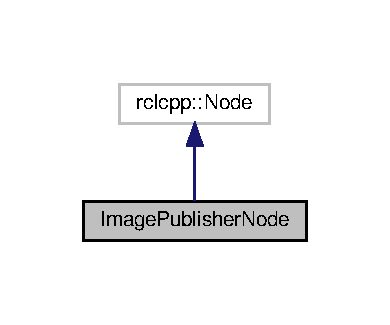
\includegraphics[width=187pt]{classImagePublisherNode__inherit__graph}
\end{center}
\end{figure}


Collaboration diagram for Image\+Publisher\+Node\+:
\nopagebreak
\begin{figure}[H]
\begin{center}
\leavevmode
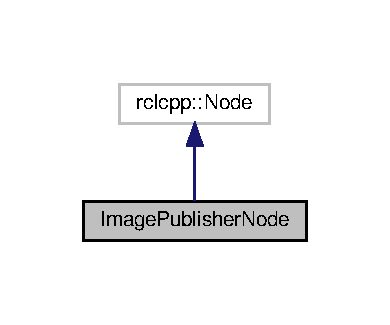
\includegraphics[width=187pt]{classImagePublisherNode__coll__graph}
\end{center}
\end{figure}
\subsection*{Private Member Functions}
\begin{DoxyCompactItemize}
\item 
\mbox{\Hypertarget{classImagePublisherNode_a28d8c880f34aa4ff0fe12f9a83db775e}\label{classImagePublisherNode_a28d8c880f34aa4ff0fe12f9a83db775e}} 
void {\bfseries publish\+Image} ()
\end{DoxyCompactItemize}
\subsection*{Private Attributes}
\begin{DoxyCompactItemize}
\item 
\mbox{\Hypertarget{classImagePublisherNode_a4346453ae3684b1898c4821de29dd19b}\label{classImagePublisherNode_a4346453ae3684b1898c4821de29dd19b}} 
rclcpp\+::\+Timer\+Base\+::\+Shared\+Ptr {\bfseries timer\+\_\+}
\item 
\mbox{\Hypertarget{classImagePublisherNode_a290f9c65a7b80a16f239b7976a956fa8}\label{classImagePublisherNode_a290f9c65a7b80a16f239b7976a956fa8}} 
rclcpp\+::\+Publisher$<$ sensor\+\_\+msgs\+::msg\+::\+Image $>$\+::Shared\+Ptr {\bfseries image\+\_\+pub\+\_\+}
\end{DoxyCompactItemize}


The documentation for this class was generated from the following files\+:\begin{DoxyCompactItemize}
\item 
lane\+\_\+keeping\+\_\+ws/src/image\+\_\+publisher/includes/Image\+Publisher\+Node.\+hpp\item 
lane\+\_\+keeping\+\_\+ws/src/image\+\_\+publisher/src/Image\+Publisher\+Node.\+cpp\end{DoxyCompactItemize}

\hypertarget{classInferenceEngine}{}\section{Inference\+Engine Class Reference}
\label{classInferenceEngine}\index{Inference\+Engine@{Inference\+Engine}}


Encapsulates Tensor\+RT engine creation, memory management, and inference execution.  




{\ttfamily \#include $<$Inference\+Engine.\+hpp$>$}

\subsection*{Public Member Functions}
\begin{DoxyCompactItemize}
\item 
\hyperlink{classInferenceEngine_a78f278f19b88965dd3bdfb24f5fa1d55}{Inference\+Engine} (std\+::shared\+\_\+ptr$<$ rclcpp\+::\+Node $>$)
\begin{DoxyCompactList}\small\item\em Construct a new \hyperlink{classInferenceEngine}{Inference\+Engine} object. \end{DoxyCompactList}\item 
bool \hyperlink{classInferenceEngine_a6319576a8a3ed00e735f7996cf4e6a48}{init} ()
\begin{DoxyCompactList}\small\item\em Initializes the inference engine\+: loads the serialized engine, creates context, and allocates memory. \end{DoxyCompactList}\item 
bool \hyperlink{classInferenceEngine_aef205091b7d9dd1614e17765c5549144}{run\+Inference} (const std\+::vector$<$ float $>$ \&flat\+\_\+img) const
\begin{DoxyCompactList}\small\item\em Runs inference on the G\+PU. \end{DoxyCompactList}\item 
float $\ast$ \hyperlink{classInferenceEngine_a4d28ceb717d506d3984dc5742dec831d}{get\+Output\+Device\+Ptr} () const
\begin{DoxyCompactList}\small\item\em Returns a pointer to the G\+PU memory containing inference results. \end{DoxyCompactList}\end{DoxyCompactItemize}
\subsection*{Private Member Functions}
\begin{DoxyCompactItemize}
\item 
I\+Cuda\+Engine $\ast$ \hyperlink{classInferenceEngine_a5f66425c0553c541353a634f991c1c00}{create\+Cuda\+Engine} ()
\begin{DoxyCompactList}\small\item\em Deserializes the engine from a precompiled engine file. \end{DoxyCompactList}\item 
void \hyperlink{classInferenceEngine_a3937cf84f22d0652cd5fe734d9b92290}{allocate\+Devices} ()
\begin{DoxyCompactList}\small\item\em Allocates C\+U\+DA device memory for input and output bindings. \end{DoxyCompactList}\end{DoxyCompactItemize}
\subsection*{Private Attributes}
\begin{DoxyCompactItemize}
\item 
\mbox{\Hypertarget{classInferenceEngine_a6f9115552d34f667591bbe5ad1c3df2a}\label{classInferenceEngine_a6f9115552d34f667591bbe5ad1c3df2a}} 
std\+::shared\+\_\+ptr$<$ rclcpp\+::\+Node $>$ {\bfseries node\+\_\+ptr\+\_\+}
\item 
\mbox{\Hypertarget{classInferenceEngine_a356266bb3a4b5caa98bb5e1302e8160b}\label{classInferenceEngine_a356266bb3a4b5caa98bb5e1302e8160b}} 
Trt\+Unique\+Ptr$<$ I\+Runtime $>$ {\bfseries runtime\+\_\+}
\item 
\mbox{\Hypertarget{classInferenceEngine_a89a6c2706b1cab79fd9eacf5cd7f82be}\label{classInferenceEngine_a89a6c2706b1cab79fd9eacf5cd7f82be}} 
Trt\+Unique\+Ptr$<$ I\+Execution\+Context $>$ {\bfseries context\+\_\+}
\item 
\mbox{\Hypertarget{classInferenceEngine_a1e7992d16fe4b5e25eef0517ec67bccd}\label{classInferenceEngine_a1e7992d16fe4b5e25eef0517ec67bccd}} 
Trt\+Unique\+Ptr$<$ I\+Cuda\+Engine $>$ {\bfseries engine\+\_\+}
\item 
\mbox{\Hypertarget{classInferenceEngine_af0697224adebb8e40690a83db827d248}\label{classInferenceEngine_af0697224adebb8e40690a83db827d248}} 
size\+\_\+t {\bfseries input\+\_\+size\+\_\+} \{1\}
\item 
\mbox{\Hypertarget{classInferenceEngine_ac88b59cb61f651e6aedb8767f78c2437}\label{classInferenceEngine_ac88b59cb61f651e6aedb8767f78c2437}} 
size\+\_\+t {\bfseries output\+\_\+size\+\_\+} \{1\}
\item 
\mbox{\Hypertarget{classInferenceEngine_a7f9db5fbd5c9fc93ac1d09e8b41c4b1f}\label{classInferenceEngine_a7f9db5fbd5c9fc93ac1d09e8b41c4b1f}} 
Cuda\+Unique\+Ptr$<$ void $>$ {\bfseries d\+\_\+input\+\_\+}
\item 
\mbox{\Hypertarget{classInferenceEngine_aada91220d42a1650c76797f95dc3089f}\label{classInferenceEngine_aada91220d42a1650c76797f95dc3089f}} 
Cuda\+Unique\+Ptr$<$ void $>$ {\bfseries d\+\_\+output\+\_\+}
\end{DoxyCompactItemize}


\subsection{Detailed Description}
Encapsulates Tensor\+RT engine creation, memory management, and inference execution. 

This class manages the full lifecycle of the Tensor\+RT engine, including deserialization, context creation, device memory allocation, and inference execution. The inference result is kept on the G\+PU to allow efficient post-\/processing. 

\subsection{Constructor \& Destructor Documentation}
\mbox{\Hypertarget{classInferenceEngine_a78f278f19b88965dd3bdfb24f5fa1d55}\label{classInferenceEngine_a78f278f19b88965dd3bdfb24f5fa1d55}} 
\index{Inference\+Engine@{Inference\+Engine}!Inference\+Engine@{Inference\+Engine}}
\index{Inference\+Engine@{Inference\+Engine}!Inference\+Engine@{Inference\+Engine}}
\subsubsection{\texorpdfstring{Inference\+Engine()}{InferenceEngine()}}
{\footnotesize\ttfamily Inference\+Engine\+::\+Inference\+Engine (\begin{DoxyParamCaption}\item[{std\+::shared\+\_\+ptr$<$ rclcpp\+::\+Node $>$}]{node\+\_\+ptr }\end{DoxyParamCaption})}



Construct a new \hyperlink{classInferenceEngine}{Inference\+Engine} object. 


\begin{DoxyParams}{Parameters}
{\em node\+\_\+ptr} & Shared R\+O\+S2 node pointer used for logging and context. \\
\hline
\end{DoxyParams}


\subsection{Member Function Documentation}
\mbox{\Hypertarget{classInferenceEngine_a3937cf84f22d0652cd5fe734d9b92290}\label{classInferenceEngine_a3937cf84f22d0652cd5fe734d9b92290}} 
\index{Inference\+Engine@{Inference\+Engine}!allocate\+Devices@{allocate\+Devices}}
\index{allocate\+Devices@{allocate\+Devices}!Inference\+Engine@{Inference\+Engine}}
\subsubsection{\texorpdfstring{allocate\+Devices()}{allocateDevices()}}
{\footnotesize\ttfamily void Inference\+Engine\+::allocate\+Devices (\begin{DoxyParamCaption}{ }\end{DoxyParamCaption})\hspace{0.3cm}{\ttfamily [private]}}



Allocates C\+U\+DA device memory for input and output bindings. 

Uses dimensions from the engine\textquotesingle{}s bindings and wraps raw allocations in smart pointers with custom deleters. \mbox{\Hypertarget{classInferenceEngine_a5f66425c0553c541353a634f991c1c00}\label{classInferenceEngine_a5f66425c0553c541353a634f991c1c00}} 
\index{Inference\+Engine@{Inference\+Engine}!create\+Cuda\+Engine@{create\+Cuda\+Engine}}
\index{create\+Cuda\+Engine@{create\+Cuda\+Engine}!Inference\+Engine@{Inference\+Engine}}
\subsubsection{\texorpdfstring{create\+Cuda\+Engine()}{createCudaEngine()}}
{\footnotesize\ttfamily I\+Cuda\+Engine $\ast$ Inference\+Engine\+::create\+Cuda\+Engine (\begin{DoxyParamCaption}{ }\end{DoxyParamCaption})\hspace{0.3cm}{\ttfamily [private]}}



Deserializes the engine from a precompiled engine file. 

\begin{DoxyReturn}{Returns}
Pointer to the created I\+Cuda\+Engine object. 
\end{DoxyReturn}
\mbox{\Hypertarget{classInferenceEngine_a4d28ceb717d506d3984dc5742dec831d}\label{classInferenceEngine_a4d28ceb717d506d3984dc5742dec831d}} 
\index{Inference\+Engine@{Inference\+Engine}!get\+Output\+Device\+Ptr@{get\+Output\+Device\+Ptr}}
\index{get\+Output\+Device\+Ptr@{get\+Output\+Device\+Ptr}!Inference\+Engine@{Inference\+Engine}}
\subsubsection{\texorpdfstring{get\+Output\+Device\+Ptr()}{getOutputDevicePtr()}}
{\footnotesize\ttfamily float $\ast$ Inference\+Engine\+::get\+Output\+Device\+Ptr (\begin{DoxyParamCaption}{ }\end{DoxyParamCaption}) const}



Returns a pointer to the G\+PU memory containing inference results. 

This allows the post-\/processing pipeline to operate directly on G\+PU memory, avoiding unnecessary memory copies.

\begin{DoxyReturn}{Returns}
float$\ast$ Pointer to device memory containing the output tensor. 
\end{DoxyReturn}
\mbox{\Hypertarget{classInferenceEngine_a6319576a8a3ed00e735f7996cf4e6a48}\label{classInferenceEngine_a6319576a8a3ed00e735f7996cf4e6a48}} 
\index{Inference\+Engine@{Inference\+Engine}!init@{init}}
\index{init@{init}!Inference\+Engine@{Inference\+Engine}}
\subsubsection{\texorpdfstring{init()}{init()}}
{\footnotesize\ttfamily bool Inference\+Engine\+::init (\begin{DoxyParamCaption}{ }\end{DoxyParamCaption})}



Initializes the inference engine\+: loads the serialized engine, creates context, and allocates memory. 

\begin{DoxyReturn}{Returns}
true if all components were successfully initialized, false otherwise. 
\end{DoxyReturn}
\mbox{\Hypertarget{classInferenceEngine_aef205091b7d9dd1614e17765c5549144}\label{classInferenceEngine_aef205091b7d9dd1614e17765c5549144}} 
\index{Inference\+Engine@{Inference\+Engine}!run\+Inference@{run\+Inference}}
\index{run\+Inference@{run\+Inference}!Inference\+Engine@{Inference\+Engine}}
\subsubsection{\texorpdfstring{run\+Inference()}{runInference()}}
{\footnotesize\ttfamily bool Inference\+Engine\+::run\+Inference (\begin{DoxyParamCaption}\item[{const std\+::vector$<$ float $>$ \&}]{flat\+\_\+img }\end{DoxyParamCaption}) const}



Runs inference on the G\+PU. 

The input image must be a flattened vector of floats. The result is stored on the G\+PU, and can be retrieved via \hyperlink{classInferenceEngine_a4d28ceb717d506d3984dc5742dec831d}{get\+Output\+Device\+Ptr()}.


\begin{DoxyParams}{Parameters}
{\em flat\+\_\+img} & Flattened input image. \\
\hline
\end{DoxyParams}
\begin{DoxyReturn}{Returns}
true if inference executed successfully, false if it failed. 
\end{DoxyReturn}


The documentation for this class was generated from the following files\+:\begin{DoxyCompactItemize}
\item 
lane\+\_\+keeping\+\_\+ws/src/ml\+\_\+vision/includes/Inference\+Engine.\+hpp\item 
lane\+\_\+keeping\+\_\+ws/src/ml\+\_\+vision/src/Inference\+Engine.\+cpp\end{DoxyCompactItemize}

\hypertarget{classKalmanFilter}{}\section{Kalman\+Filter Class Reference}
\label{classKalmanFilter}\index{Kalman\+Filter@{Kalman\+Filter}}


1d Kalman filter.  




{\ttfamily \#include $<$Kalman\+Filter.\+hpp$>$}

\subsection*{Public Member Functions}
\begin{DoxyCompactItemize}
\item 
\mbox{\Hypertarget{classKalmanFilter_a1896074df3e88eb15435cef16cb44244}\label{classKalmanFilter_a1896074df3e88eb15435cef16cb44244}} 
{\bfseries Kalman\+Filter} (double process\+\_\+variance\+\_\+, double measurement\+\_\+variance)
\item 
double \hyperlink{classKalmanFilter_ae57452f04b28846c9b68c5887eafa00e}{update} (double lane\+\_\+center)
\begin{DoxyCompactList}\small\item\em Stabilize the measurements of lane center. \end{DoxyCompactList}\end{DoxyCompactItemize}
\subsection*{Private Attributes}
\begin{DoxyCompactItemize}
\item 
\mbox{\Hypertarget{classKalmanFilter_a5fb5caac98ba62747c94b986f7524c75}\label{classKalmanFilter_a5fb5caac98ba62747c94b986f7524c75}} 
double {\bfseries x\+\_\+}
\item 
\mbox{\Hypertarget{classKalmanFilter_a4698f5f4b8ef83d799b1bcdaa87a980b}\label{classKalmanFilter_a4698f5f4b8ef83d799b1bcdaa87a980b}} 
double {\bfseries p\+\_\+}
\item 
\mbox{\Hypertarget{classKalmanFilter_ae03f4ed668e9a6b89c72e661b17de6a5}\label{classKalmanFilter_ae03f4ed668e9a6b89c72e661b17de6a5}} 
double {\bfseries q\+\_\+}
\item 
\mbox{\Hypertarget{classKalmanFilter_a65fba3cea5655017378f967838a3b0c5}\label{classKalmanFilter_a65fba3cea5655017378f967838a3b0c5}} 
double {\bfseries r\+\_\+}
\item 
\mbox{\Hypertarget{classKalmanFilter_a1ef5d7bce9ef78523004e655ccf98a5e}\label{classKalmanFilter_a1ef5d7bce9ef78523004e655ccf98a5e}} 
double {\bfseries k\+\_\+}
\end{DoxyCompactItemize}


\subsection{Detailed Description}
1d Kalman filter. 

this filter helps smooth out noisy lane center measurements. If a single camera frame has an outlier measurement,the filter will \char`\"{}trust\char`\"{} this measurement less than the prediction based on previous frames, resulting in smoother control.

process\+\_\+variance / q\+\_\+ \+: How much true lane center might change between frames measurement\+\_\+variance / r\+\_\+\+: How noisy our lane detection is

higher r\+\_\+\+: More smoothing, slower response higher q\+\_\+\+: faster response, less smoothing 

\subsection{Member Function Documentation}
\mbox{\Hypertarget{classKalmanFilter_ae57452f04b28846c9b68c5887eafa00e}\label{classKalmanFilter_ae57452f04b28846c9b68c5887eafa00e}} 
\index{Kalman\+Filter@{Kalman\+Filter}!update@{update}}
\index{update@{update}!Kalman\+Filter@{Kalman\+Filter}}
\subsubsection{\texorpdfstring{update()}{update()}}
{\footnotesize\ttfamily double Kalman\+Filter\+::update (\begin{DoxyParamCaption}\item[{double}]{lane\+\_\+center }\end{DoxyParamCaption})}



Stabilize the measurements of lane center. 

the filtering is done in steps\+:
\begin{DoxyItemize}
\item prediction\+: increase uncertainty by adding process noise
\item Calculate kalman gain\+: How much do we trust the prediction
\item correct the measurement with uncertainty and gain.
\item Update uncertainty\+: the closer prediction and measurement are the smaller this value gets
\end{DoxyItemize}


\begin{DoxyParams}{Parameters}
{\em lane\+\_\+center} & \\
\hline
\end{DoxyParams}
\begin{DoxyReturn}{Returns}

\end{DoxyReturn}


The documentation for this class was generated from the following files\+:\begin{DoxyCompactItemize}
\item 
lane\+\_\+keeping\+\_\+ws/src/motion\+\_\+control/includes/Kalman\+Filter.\+hpp\item 
lane\+\_\+keeping\+\_\+ws/src/motion\+\_\+control/src/Kalman\+Filter.\+cpp\end{DoxyCompactItemize}

\hypertarget{classLaneBuffer}{}\section{Lane\+Buffer Class Reference}
\label{classLaneBuffer}\index{Lane\+Buffer@{Lane\+Buffer}}
\subsection*{Public Member Functions}
\begin{DoxyCompactItemize}
\item 
\mbox{\Hypertarget{classLaneBuffer_a28001137e1ad1e0364d60d747e76c96e}\label{classLaneBuffer_a28001137e1ad1e0364d60d747e76c96e}} 
{\bfseries Lane\+Buffer} (size\+\_\+t max\+\_\+size)
\item 
\mbox{\Hypertarget{classLaneBuffer_aace7ec7b4c42278ee7fa628133308e6e}\label{classLaneBuffer_aace7ec7b4c42278ee7fa628133308e6e}} 
std\+::vector$<$ double $>$ {\bfseries get\+Last\+Left} ()
\item 
\mbox{\Hypertarget{classLaneBuffer_a2b7ad2f7ce41a723eaaf75aa11af16c4}\label{classLaneBuffer_a2b7ad2f7ce41a723eaaf75aa11af16c4}} 
std\+::vector$<$ double $>$ {\bfseries get\+Last\+Right} ()
\item 
\mbox{\Hypertarget{classLaneBuffer_a14620e6321b73076f67ddff2dd751da0}\label{classLaneBuffer_a14620e6321b73076f67ddff2dd751da0}} 
void {\bfseries add\+Coeffs} (std\+::vector$<$ double $>$ \&left\+\_\+coefs, std\+::vector$<$ double $>$ \&right\+\_\+coefs)
\item 
\mbox{\Hypertarget{classLaneBuffer_a1fef01a11888d2ecbd9b4fea74a804e6}\label{classLaneBuffer_a1fef01a11888d2ecbd9b4fea74a804e6}} 
bool {\bfseries has\+Left\+Lane} ()
\item 
\mbox{\Hypertarget{classLaneBuffer_a209a951ff1fe55079eb5b8554c55b93d}\label{classLaneBuffer_a209a951ff1fe55079eb5b8554c55b93d}} 
bool {\bfseries has\+Right\+Lane} ()
\item 
\mbox{\Hypertarget{classLaneBuffer_a3cf22e3f47f14a851a99686fcdc35cfe}\label{classLaneBuffer_a3cf22e3f47f14a851a99686fcdc35cfe}} 
size\+\_\+t {\bfseries get\+Left\+Size} ()
\item 
\mbox{\Hypertarget{classLaneBuffer_a8d9c5d68d724bcacbe96092d98fc6ad1}\label{classLaneBuffer_a8d9c5d68d724bcacbe96092d98fc6ad1}} 
size\+\_\+t {\bfseries get\+Right\+Size} ()
\end{DoxyCompactItemize}
\subsection*{Private Attributes}
\begin{DoxyCompactItemize}
\item 
\mbox{\Hypertarget{classLaneBuffer_afabb27169371ebf7b9ecec0bc6ac9757}\label{classLaneBuffer_afabb27169371ebf7b9ecec0bc6ac9757}} 
size\+\_\+t {\bfseries max\+\_\+size\+\_\+}
\item 
\mbox{\Hypertarget{classLaneBuffer_a04a15a527a56822527ede138f916d23a}\label{classLaneBuffer_a04a15a527a56822527ede138f916d23a}} 
std\+::deque$<$ std\+::vector$<$ double $>$ $>$ {\bfseries left\+\_\+lane\+\_\+}
\item 
\mbox{\Hypertarget{classLaneBuffer_abb489a9391c6013769600f0433ab80dc}\label{classLaneBuffer_abb489a9391c6013769600f0433ab80dc}} 
std\+::deque$<$ std\+::vector$<$ double $>$ $>$ {\bfseries right\+\_\+lane\+\_\+}
\end{DoxyCompactItemize}


The documentation for this class was generated from the following files\+:\begin{DoxyCompactItemize}
\item 
lane\+\_\+keeping\+\_\+ws/src/motion\+\_\+control/includes/Lane\+Buffer.\+hpp\item 
lane\+\_\+keeping\+\_\+ws/src/motion\+\_\+control/src/Lane\+Buffer.\+cpp\end{DoxyCompactItemize}

\hypertarget{classLaneBufferTest}{}\section{Lane\+Buffer\+Test Class Reference}
\label{classLaneBufferTest}\index{Lane\+Buffer\+Test@{Lane\+Buffer\+Test}}


Inheritance diagram for Lane\+Buffer\+Test\+:
\nopagebreak
\begin{figure}[H]
\begin{center}
\leavevmode
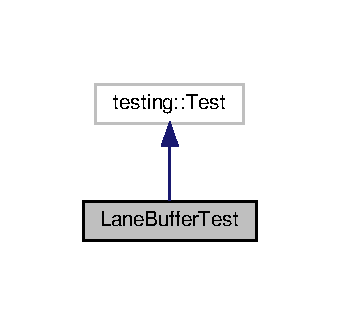
\includegraphics[width=163pt]{classLaneBufferTest__inherit__graph}
\end{center}
\end{figure}


Collaboration diagram for Lane\+Buffer\+Test\+:
\nopagebreak
\begin{figure}[H]
\begin{center}
\leavevmode
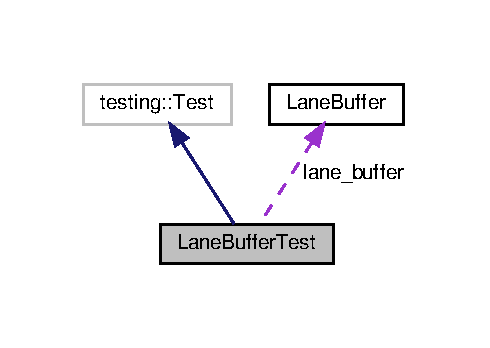
\includegraphics[width=235pt]{classLaneBufferTest__coll__graph}
\end{center}
\end{figure}
\subsection*{Protected Attributes}
\begin{DoxyCompactItemize}
\item 
\mbox{\Hypertarget{classLaneBufferTest_a394943c7852ef49fd6abad2ed77ff7b2}\label{classLaneBufferTest_a394943c7852ef49fd6abad2ed77ff7b2}} 
\hyperlink{classLaneBuffer}{Lane\+Buffer} {\bfseries lane\+\_\+buffer}
\end{DoxyCompactItemize}


The documentation for this class was generated from the following file\+:\begin{DoxyCompactItemize}
\item 
lane\+\_\+keeping\+\_\+ws/src/motion\+\_\+control/test/src/Lane\+Buffer\+Test.\+cpp\end{DoxyCompactItemize}

\hypertarget{classLaneVisualizationNode}{}\section{Lane\+Visualization\+Node Class Reference}
\label{classLaneVisualizationNode}\index{Lane\+Visualization\+Node@{Lane\+Visualization\+Node}}


Display the geometries published by the vision and motion node (lane positions, polyfits...)  




{\ttfamily \#include $<$Lane\+Visualization\+Node.\+hpp$>$}



Inheritance diagram for Lane\+Visualization\+Node\+:
\nopagebreak
\begin{figure}[H]
\begin{center}
\leavevmode
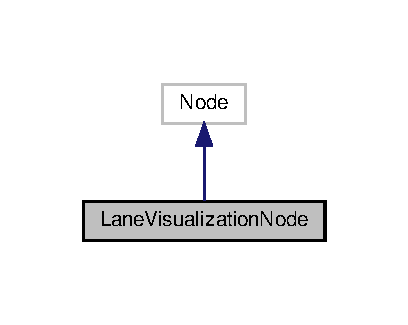
\includegraphics[width=196pt]{classLaneVisualizationNode__inherit__graph}
\end{center}
\end{figure}


Collaboration diagram for Lane\+Visualization\+Node\+:
\nopagebreak
\begin{figure}[H]
\begin{center}
\leavevmode
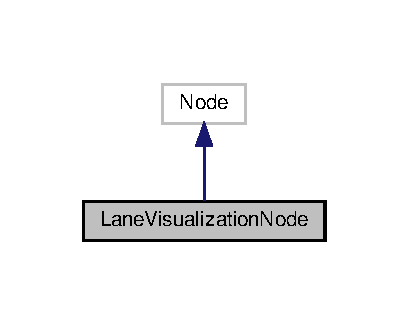
\includegraphics[width=196pt]{classLaneVisualizationNode__coll__graph}
\end{center}
\end{figure}
\subsection*{Public Member Functions}
\begin{DoxyCompactItemize}
\item 
\mbox{\Hypertarget{classLaneVisualizationNode_adfe0bf0212e85e99558d4b7ce462383d}\label{classLaneVisualizationNode_adfe0bf0212e85e99558d4b7ce462383d}} 
void {\bfseries init\+Publishers} ()
\end{DoxyCompactItemize}
\subsection*{Private Member Functions}
\begin{DoxyCompactItemize}
\item 
void \hyperlink{classLaneVisualizationNode_a659b897bbab6410ac46e7ada948b7de2}{raw\+Image\+Callback} (const sensor\+\_\+msgs\+::msg\+::\+Image\+::\+Shared\+Ptr msg)
\begin{DoxyCompactList}\small\item\em callback for raw image subscriber. \end{DoxyCompactList}\item 
\mbox{\Hypertarget{classLaneVisualizationNode_acc79d01a5c9f6ef2d3028742376c389d}\label{classLaneVisualizationNode_acc79d01a5c9f6ef2d3028742376c389d}} 
void {\bfseries store\+Lane\+Position} (const lane\+\_\+msgs\+::msg\+::\+Lane\+Positions\+::\+Shared\+Ptr msg)
\item 
\mbox{\Hypertarget{classLaneVisualizationNode_a94d31de5b98a84e8d47113f57071edc8}\label{classLaneVisualizationNode_a94d31de5b98a84e8d47113f57071edc8}} 
void {\bfseries store\+Coefs} (const lane\+\_\+msgs\+::msg\+::\+Polyfit\+Coefs\+::\+Shared\+Ptr msg)
\end{DoxyCompactItemize}
\subsection*{Private Attributes}
\begin{DoxyCompactItemize}
\item 
\mbox{\Hypertarget{classLaneVisualizationNode_a268dac1df1b6c937091db71f441f0e5c}\label{classLaneVisualizationNode_a268dac1df1b6c937091db71f441f0e5c}} 
std\+::vector$<$ double $>$ {\bfseries left\+\_\+coefs\+\_\+}
\item 
\mbox{\Hypertarget{classLaneVisualizationNode_ae25334f837d5d7af1f757d531dfd0686}\label{classLaneVisualizationNode_ae25334f837d5d7af1f757d531dfd0686}} 
std\+::vector$<$ double $>$ {\bfseries right\+\_\+coefs\+\_\+}
\item 
\mbox{\Hypertarget{classLaneVisualizationNode_ad26b5a0a84fc70c42d96e5246e65d41e}\label{classLaneVisualizationNode_ad26b5a0a84fc70c42d96e5246e65d41e}} 
std\+::vector$<$ Point32 $>$ {\bfseries left\+\_\+lane\+\_\+pos\+\_\+}
\item 
\mbox{\Hypertarget{classLaneVisualizationNode_ab0d648873fb5260b77f5198875dceeab}\label{classLaneVisualizationNode_ab0d648873fb5260b77f5198875dceeab}} 
std\+::vector$<$ Point32 $>$ {\bfseries right\+\_\+lane\+\_\+pos\+\_\+}
\item 
\mbox{\Hypertarget{classLaneVisualizationNode_a1770f42de616c7fb867ce19d3e495201}\label{classLaneVisualizationNode_a1770f42de616c7fb867ce19d3e495201}} 
Point32 {\bfseries lane\+\_\+center\+\_\+}
\item 
\mbox{\Hypertarget{classLaneVisualizationNode_ab6687133edfd3067fea8c7aec91f97bc}\label{classLaneVisualizationNode_ab6687133edfd3067fea8c7aec91f97bc}} 
rclcpp\+::\+Subscription$<$ sensor\+\_\+msgs\+::msg\+::\+Image $>$\+::Shared\+Ptr {\bfseries raw\+\_\+img\+\_\+sub\+\_\+}
\item 
\mbox{\Hypertarget{classLaneVisualizationNode_ae2e8d02bfc45db689c05c130f2ae65bd}\label{classLaneVisualizationNode_ae2e8d02bfc45db689c05c130f2ae65bd}} 
rclcpp\+::\+Subscription$<$ lane\+\_\+msgs\+::msg\+::\+Lane\+Positions $>$\+::Shared\+Ptr {\bfseries lane\+\_\+pos\+\_\+sub\+\_\+}
\item 
\mbox{\Hypertarget{classLaneVisualizationNode_a42495fb3f3a4e1a7da23a3baa7a0b709}\label{classLaneVisualizationNode_a42495fb3f3a4e1a7da23a3baa7a0b709}} 
rclcpp\+::\+Subscription$<$ lane\+\_\+msgs\+::msg\+::\+Polyfit\+Coefs $>$\+::Shared\+Ptr {\bfseries polyfit\+\_\+coefs\+\_\+sub\+\_\+}
\item 
\mbox{\Hypertarget{classLaneVisualizationNode_aaf4b2b01423616d3333f3c69915c736f}\label{classLaneVisualizationNode_aaf4b2b01423616d3333f3c69915c736f}} 
image\+\_\+transport\+::\+Publisher {\bfseries processed\+\_\+img\+\_\+pub\+\_\+}
\end{DoxyCompactItemize}


\subsection{Detailed Description}
Display the geometries published by the vision and motion node (lane positions, polyfits...) 

Subscribe to lane position and polyfit coefficient. When new values arrive, they are stored in member variables. Subscribe to raw\+\_\+image, draws the stored geometries on the orignal picture and publish the result in processed\+\_\+img. 

\subsection{Member Function Documentation}
\mbox{\Hypertarget{classLaneVisualizationNode_a659b897bbab6410ac46e7ada948b7de2}\label{classLaneVisualizationNode_a659b897bbab6410ac46e7ada948b7de2}} 
\index{Lane\+Visualization\+Node@{Lane\+Visualization\+Node}!raw\+Image\+Callback@{raw\+Image\+Callback}}
\index{raw\+Image\+Callback@{raw\+Image\+Callback}!Lane\+Visualization\+Node@{Lane\+Visualization\+Node}}
\subsubsection{\texorpdfstring{raw\+Image\+Callback()}{rawImageCallback()}}
{\footnotesize\ttfamily void Lane\+Visualization\+Node\+::raw\+Image\+Callback (\begin{DoxyParamCaption}\item[{const sensor\+\_\+msgs\+::msg\+::\+Image\+::\+Shared\+Ptr}]{msg }\end{DoxyParamCaption})\hspace{0.3cm}{\ttfamily [private]}}



callback for raw image subscriber. 

Called upon receiving a new image. responsible for drawing all the features extracted by our algorithms (lane points, polylines...) onto the original image. publishes the result processed\+\_\+img.


\begin{DoxyParams}{Parameters}
{\em msg} & \\
\hline
\end{DoxyParams}


The documentation for this class was generated from the following files\+:\begin{DoxyCompactItemize}
\item 
lane\+\_\+keeping\+\_\+ws/src/lane\+\_\+visualization/includes/Lane\+Visualization\+Node.\+hpp\item 
lane\+\_\+keeping\+\_\+ws/src/lane\+\_\+visualization/src/Lane\+Visualization\+Node.\+cpp\end{DoxyCompactItemize}

\hypertarget{classLogger}{}\section{Logger Class Reference}
\label{classLogger}\index{Logger@{Logger}}


Inheritance diagram for Logger\+:
\nopagebreak
\begin{figure}[H]
\begin{center}
\leavevmode
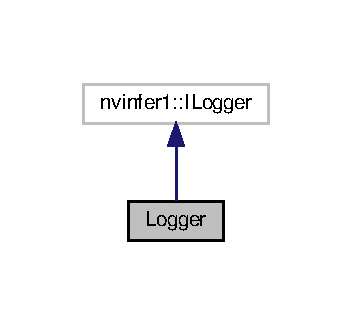
\includegraphics[width=169pt]{classLogger__inherit__graph}
\end{center}
\end{figure}


Collaboration diagram for Logger\+:
\nopagebreak
\begin{figure}[H]
\begin{center}
\leavevmode
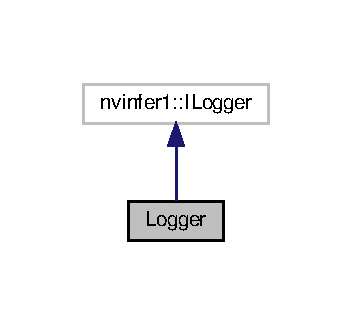
\includegraphics[width=169pt]{classLogger__coll__graph}
\end{center}
\end{figure}
\subsection*{Private Member Functions}
\begin{DoxyCompactItemize}
\item 
\mbox{\Hypertarget{classLogger_a2d536d8a8c1354c2ff1236efe6a395ff}\label{classLogger_a2d536d8a8c1354c2ff1236efe6a395ff}} 
void {\bfseries log} (Severity severity, const char $\ast$msg) noexcept override
\end{DoxyCompactItemize}


The documentation for this class was generated from the following files\+:\begin{DoxyCompactItemize}
\item 
lane\+\_\+keeping\+\_\+ws/src/ml\+\_\+vision/includes/Logger.\+hpp\item 
lane\+\_\+keeping\+\_\+ws/src/ml\+\_\+vision/src/Logger.\+cpp\end{DoxyCompactItemize}

\hypertarget{classMlVisionNode}{}\section{Ml\+Vision\+Node Class Reference}
\label{classMlVisionNode}\index{Ml\+Vision\+Node@{Ml\+Vision\+Node}}


Performs lane detection using a deep learning model accelerated with Tensor\+RT and C\+U\+D\+A-\/based image preprocessing.  




{\ttfamily \#include $<$Ml\+Vision\+Node.\+hpp$>$}



Inheritance diagram for Ml\+Vision\+Node\+:
\nopagebreak
\begin{figure}[H]
\begin{center}
\leavevmode
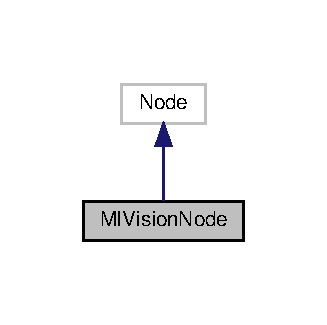
\includegraphics[width=157pt]{classMlVisionNode__inherit__graph}
\end{center}
\end{figure}


Collaboration diagram for Ml\+Vision\+Node\+:
\nopagebreak
\begin{figure}[H]
\begin{center}
\leavevmode
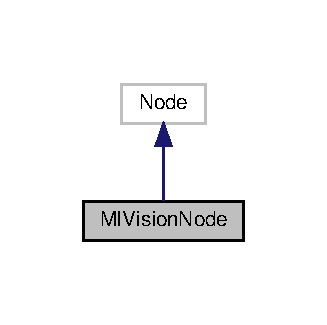
\includegraphics[width=157pt]{classMlVisionNode__coll__graph}
\end{center}
\end{figure}
\subsection*{Public Member Functions}
\begin{DoxyCompactItemize}
\item 
\mbox{\Hypertarget{classMlVisionNode_a1a07ccd1830082c3e28ff97f95819618}\label{classMlVisionNode_a1a07ccd1830082c3e28ff97f95819618}} 
\hyperlink{classMlVisionNode_a1a07ccd1830082c3e28ff97f95819618}{Ml\+Vision\+Node} ()
\begin{DoxyCompactList}\small\item\em Initialize R\+OS subscriber and publisher as well as Open\+CV objects used for post processing of inference output. \end{DoxyCompactList}\item 
bool \hyperlink{classMlVisionNode_aadb64eb869ae730fa6766f95d3c352a2}{init} ()
\begin{DoxyCompactList}\small\item\em Initializes inference engine, image processor, and debug publishers. \end{DoxyCompactList}\end{DoxyCompactItemize}
\subsection*{Private Member Functions}
\begin{DoxyCompactItemize}
\item 
void \hyperlink{classMlVisionNode_a1926f7a99c102f89f739240ecd44f6e7}{raw\+Image\+Callback} (sensor\+\_\+msgs\+::msg\+::\+Image\+::\+Shared\+Ptr img\+\_\+msg)
\begin{DoxyCompactList}\small\item\em Callback for raw camera image subscription. \end{DoxyCompactList}\item 
void \hyperlink{classMlVisionNode_a508766f7ec927847d5ce80abd9740c7c}{publish\+Lane\+Positions} (std\+::vector$<$ cv\+::\+Vec4i $>$ \&lines)
\begin{DoxyCompactList}\small\item\em Publishes detected lane line segments as R\+OS message. \end{DoxyCompactList}\item 
void \hyperlink{classMlVisionNode_a56422aa2b6f2843226bdeff85ebe785f}{publish\+Debug} (cv\+::cuda\+::\+Gpu\+Mat \&gpu\+\_\+img, image\+\_\+transport\+::\+Publisher \&publisher) const
\begin{DoxyCompactList}\small\item\em Publishes debug image to the topic associated with the publisher passed in argument. \end{DoxyCompactList}\end{DoxyCompactItemize}
\subsection*{Private Attributes}
\begin{DoxyCompactItemize}
\item 
\mbox{\Hypertarget{classMlVisionNode_a8ebe91f1d8bcc201e24e338e9f0c4ba4}\label{classMlVisionNode_a8ebe91f1d8bcc201e24e338e9f0c4ba4}} 
rclcpp\+::\+Subscription$<$ sensor\+\_\+msgs\+::msg\+::\+Image $>$\+::Shared\+Ptr {\bfseries raw\+\_\+img\+\_\+sub\+\_\+}
\item 
\mbox{\Hypertarget{classMlVisionNode_ab2e74b44fff25866be5d3cec30b39952}\label{classMlVisionNode_ab2e74b44fff25866be5d3cec30b39952}} 
rclcpp\+::\+Publisher$<$ lane\+\_\+msgs\+::msg\+::\+Lane\+Positions $>$\+::Shared\+Ptr {\bfseries lane\+\_\+pos\+\_\+pub\+\_\+}
\item 
\mbox{\Hypertarget{classMlVisionNode_a96293498d7a32bacea2df5f43bec8251}\label{classMlVisionNode_a96293498d7a32bacea2df5f43bec8251}} 
image\+\_\+transport\+::\+Publisher {\bfseries raw\+\_\+mask\+\_\+pub\+\_\+}
\item 
\mbox{\Hypertarget{classMlVisionNode_ae419a723f4e2b5458808a5f0b714df73}\label{classMlVisionNode_ae419a723f4e2b5458808a5f0b714df73}} 
image\+\_\+transport\+::\+Publisher {\bfseries tresholded\+\_\+mask\+\_\+pub\+\_\+}
\item 
\mbox{\Hypertarget{classMlVisionNode_a4d6f6dc34bed19ce55770a7334da690f}\label{classMlVisionNode_a4d6f6dc34bed19ce55770a7334da690f}} 
image\+\_\+transport\+::\+Publisher {\bfseries edge\+\_\+mask\+\_\+pub\+\_\+}
\item 
\mbox{\Hypertarget{classMlVisionNode_a6729993d3f3b51aac48f2737d5fdadc5}\label{classMlVisionNode_a6729993d3f3b51aac48f2737d5fdadc5}} 
std\+::unique\+\_\+ptr$<$ \hyperlink{classInferenceEngine}{Inference\+Engine} $>$ {\bfseries inference\+\_\+engine\+\_\+}
\item 
\mbox{\Hypertarget{classMlVisionNode_aedc401e6a70754ff92bd7a91d2187b80}\label{classMlVisionNode_aedc401e6a70754ff92bd7a91d2187b80}} 
std\+::unique\+\_\+ptr$<$ \hyperlink{classImageProcessor}{Image\+Processor} $>$ {\bfseries image\+\_\+processor\+\_\+}
\end{DoxyCompactItemize}


\subsection{Detailed Description}
Performs lane detection using a deep learning model accelerated with Tensor\+RT and C\+U\+D\+A-\/based image preprocessing. 

Responsibilities\+:
\begin{DoxyItemize}
\item Subscribes to raw camera images.
\item Runs image preprocessing (resize, flatten).
\item Executes inference on G\+PU using Tensor\+RT.
\item Posprocess image (treshold, morpho operations, Canny edge)
\item Extracts lane lines from model output via Hough Transform.
\item Publishes lane lines and debug visualizations. 
\end{DoxyItemize}

\subsection{Member Function Documentation}
\mbox{\Hypertarget{classMlVisionNode_aadb64eb869ae730fa6766f95d3c352a2}\label{classMlVisionNode_aadb64eb869ae730fa6766f95d3c352a2}} 
\index{Ml\+Vision\+Node@{Ml\+Vision\+Node}!init@{init}}
\index{init@{init}!Ml\+Vision\+Node@{Ml\+Vision\+Node}}
\subsubsection{\texorpdfstring{init()}{init()}}
{\footnotesize\ttfamily bool Ml\+Vision\+Node\+::init (\begin{DoxyParamCaption}{ }\end{DoxyParamCaption})}



Initializes inference engine, image processor, and debug publishers. 

\begin{DoxyReturn}{Returns}
True if successful. 
\end{DoxyReturn}
\mbox{\Hypertarget{classMlVisionNode_a56422aa2b6f2843226bdeff85ebe785f}\label{classMlVisionNode_a56422aa2b6f2843226bdeff85ebe785f}} 
\index{Ml\+Vision\+Node@{Ml\+Vision\+Node}!publish\+Debug@{publish\+Debug}}
\index{publish\+Debug@{publish\+Debug}!Ml\+Vision\+Node@{Ml\+Vision\+Node}}
\subsubsection{\texorpdfstring{publish\+Debug()}{publishDebug()}}
{\footnotesize\ttfamily void Ml\+Vision\+Node\+::publish\+Debug (\begin{DoxyParamCaption}\item[{cv\+::cuda\+::\+Gpu\+Mat \&}]{gpu\+\_\+img,  }\item[{image\+\_\+transport\+::\+Publisher \&}]{publisher }\end{DoxyParamCaption}) const\hspace{0.3cm}{\ttfamily [private]}}



Publishes debug image to the topic associated with the publisher passed in argument. 


\begin{DoxyParams}{Parameters}
{\em gpu\+\_\+img} & The image to publish. \\
\hline
{\em publisher} & The publisher associated with the debug topic. \\
\hline
\end{DoxyParams}
\mbox{\Hypertarget{classMlVisionNode_a508766f7ec927847d5ce80abd9740c7c}\label{classMlVisionNode_a508766f7ec927847d5ce80abd9740c7c}} 
\index{Ml\+Vision\+Node@{Ml\+Vision\+Node}!publish\+Lane\+Positions@{publish\+Lane\+Positions}}
\index{publish\+Lane\+Positions@{publish\+Lane\+Positions}!Ml\+Vision\+Node@{Ml\+Vision\+Node}}
\subsubsection{\texorpdfstring{publish\+Lane\+Positions()}{publishLanePositions()}}
{\footnotesize\ttfamily void Ml\+Vision\+Node\+::publish\+Lane\+Positions (\begin{DoxyParamCaption}\item[{std\+::vector$<$ cv\+::\+Vec4i $>$ \&}]{lines }\end{DoxyParamCaption})\hspace{0.3cm}{\ttfamily [private]}}



Publishes detected lane line segments as R\+OS message. 


\begin{DoxyParams}{Parameters}
{\em lines} & Vector of detected lines (Vec4i format). \\
\hline
\end{DoxyParams}
\mbox{\Hypertarget{classMlVisionNode_a1926f7a99c102f89f739240ecd44f6e7}\label{classMlVisionNode_a1926f7a99c102f89f739240ecd44f6e7}} 
\index{Ml\+Vision\+Node@{Ml\+Vision\+Node}!raw\+Image\+Callback@{raw\+Image\+Callback}}
\index{raw\+Image\+Callback@{raw\+Image\+Callback}!Ml\+Vision\+Node@{Ml\+Vision\+Node}}
\subsubsection{\texorpdfstring{raw\+Image\+Callback()}{rawImageCallback()}}
{\footnotesize\ttfamily void Ml\+Vision\+Node\+::raw\+Image\+Callback (\begin{DoxyParamCaption}\item[{sensor\+\_\+msgs\+::msg\+::\+Image\+::\+Shared\+Ptr}]{img\+\_\+msg }\end{DoxyParamCaption})\hspace{0.3cm}{\ttfamily [private]}}



Callback for raw camera image subscription. 

Handles image conversion, inference, and postprocessing.


\begin{DoxyParams}{Parameters}
{\em img\+\_\+msg} & The incoming image message. \\
\hline
\end{DoxyParams}


The documentation for this class was generated from the following files\+:\begin{DoxyCompactItemize}
\item 
lane\+\_\+keeping\+\_\+ws/src/ml\+\_\+vision/includes/Ml\+Vision\+Node.\+hpp\item 
lane\+\_\+keeping\+\_\+ws/src/ml\+\_\+vision/src/Ml\+Vision\+Node.\+cpp\end{DoxyCompactItemize}

\hypertarget{classMotionControlNode}{}\section{Motion\+Control\+Node Class Reference}
\label{classMotionControlNode}\index{Motion\+Control\+Node@{Motion\+Control\+Node}}


Implements lane-\/keeping control using polynomial fitting and P\+ID control.  




{\ttfamily \#include $<$Motion\+Control\+Node.\+hpp$>$}



Inheritance diagram for Motion\+Control\+Node\+:
\nopagebreak
\begin{figure}[H]
\begin{center}
\leavevmode
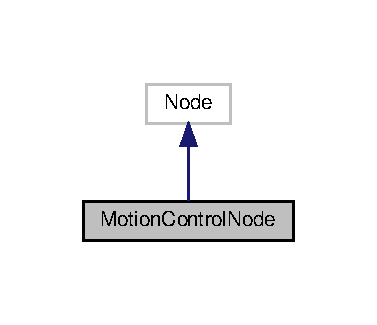
\includegraphics[width=181pt]{classMotionControlNode__inherit__graph}
\end{center}
\end{figure}


Collaboration diagram for Motion\+Control\+Node\+:
\nopagebreak
\begin{figure}[H]
\begin{center}
\leavevmode
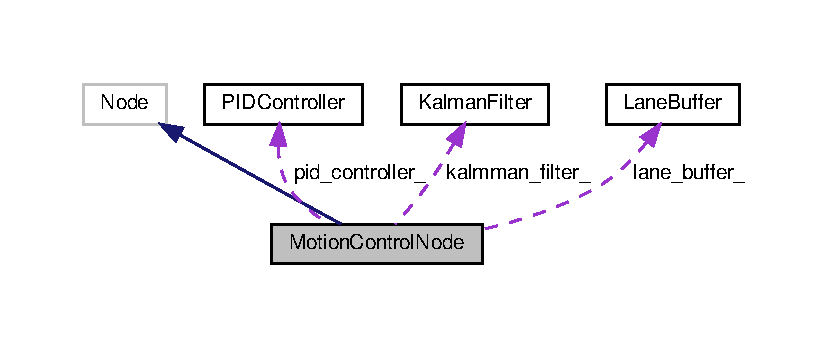
\includegraphics[width=350pt]{classMotionControlNode__coll__graph}
\end{center}
\end{figure}
\subsection*{Public Member Functions}
\begin{DoxyCompactItemize}
\item 
\hyperlink{classMotionControlNode_a2d6c4f671ad827ffce0379d8c704ffb3}{Motion\+Control\+Node} ()
\begin{DoxyCompactList}\small\item\em Initializes R\+O\+S2 subscriptions, publishers, and control parameters. \end{DoxyCompactList}\item 
\mbox{\Hypertarget{classMotionControlNode_ad1497ac89b446c40635e05da0313b922}\label{classMotionControlNode_ad1497ac89b446c40635e05da0313b922}} 
void {\bfseries init\+P\+I\+D\+Controller} ()
\end{DoxyCompactItemize}
\subsection*{Private Member Functions}
\begin{DoxyCompactItemize}
\item 
void \hyperlink{classMotionControlNode_a282a762671c7b667f174717ff0dcea20}{lane\+Position\+Callback} (lane\+\_\+msgs\+::msg\+::\+Lane\+Positions\+::\+Shared\+Ptr lane\+\_\+msg)
\begin{DoxyCompactList}\small\item\em Processes incoming lane positions and computes control commands. \end{DoxyCompactList}\item 
void \hyperlink{classMotionControlNode_a67cc5bcda286ffbe809d0555bdaf6a8d}{separate\+And\+Order\+Coordinates} (const std\+::vector$<$ Point32 $>$ \&points, std\+::vector$<$ double $>$ \&x, std\+::vector$<$ double $>$ \&y)
\begin{DoxyCompactList}\small\item\em Separates and sorts lane points by y-\/coordinate. \end{DoxyCompactList}\item 
void \hyperlink{classMotionControlNode_acab5e28f36d5a16521c38073077e2b1d}{calculate\+Polyfit\+Coefs} (std\+::vector$<$ double $>$ \&left\+\_\+coefs, std\+::vector$<$ double $>$ \&right\+\_\+coefs, lane\+\_\+msgs\+::msg\+::\+Lane\+Positions\+::\+Shared\+Ptr lane\+\_\+msg)
\begin{DoxyCompactList}\small\item\em Fits 2nd-\/degree polynomials to left/right lane points. \end{DoxyCompactList}\item 
Point32 \hyperlink{classMotionControlNode_a2c48d9d1ef7222d03c69f8dc86cd1842}{find\+Lane\+Center} (const std\+::vector$<$ double $>$ \&left\+\_\+coef, const std\+::vector$<$ double $>$ \&right\+\_\+coef, int img\+\_\+height)
\begin{DoxyCompactList}\small\item\em Computes lane center at a fixed lookahead distance. \end{DoxyCompactList}\item 
Point32 \hyperlink{classMotionControlNode_a9a30201e0d7cb92779f222c38804ec03}{find\+Heading\+Point} (int img\+\_\+width, int img\+\_\+height)
\begin{DoxyCompactList}\small\item\em Find where the car is heading using lookahead\+\_\+index parameter. \end{DoxyCompactList}\item 
void \hyperlink{classMotionControlNode_abad42e896700d175ae870d3eed4a79ea}{calculate\+And\+Publish\+Controls} (Point32 \&lane\+\_\+center, Point32 \&heading\+\_\+point, int img\+\_\+width)
\begin{DoxyCompactList}\small\item\em Computes steering command using P\+ID control. \end{DoxyCompactList}\item 
void \hyperlink{classMotionControlNode_a2f890913a81fdb965348897dbd972a77}{publish\+Polyfit\+Coefficients} (const std\+::vector$<$ double $>$ \&left\+\_\+coefs, const std\+::vector$<$ double $>$ \&right\+\_\+coefs, Point32 \&lane\+\_\+center)
\begin{DoxyCompactList}\small\item\em Publishes polynomial coefficients and lane center. \end{DoxyCompactList}\item 
\mbox{\Hypertarget{classMotionControlNode_a9ab1d5f6c9141de3c04ce19bc29e14a6}\label{classMotionControlNode_a9ab1d5f6c9141de3c04ce19bc29e14a6}} 
void {\bfseries stop\+Vehicle} ()
\end{DoxyCompactItemize}
\subsection*{Private Attributes}
\begin{DoxyCompactItemize}
\item 
\mbox{\Hypertarget{classMotionControlNode_ab153e88844739c39e94bf0ba8540251e}\label{classMotionControlNode_ab153e88844739c39e94bf0ba8540251e}} 
\hyperlink{classLaneBuffer}{Lane\+Buffer} {\bfseries lane\+\_\+buffer\+\_\+}
\item 
\mbox{\Hypertarget{classMotionControlNode_a9848ef14a93e7123e9ce374b422d7952}\label{classMotionControlNode_a9848ef14a93e7123e9ce374b422d7952}} 
\hyperlink{classPIDController}{P\+I\+D\+Controller} {\bfseries pid\+\_\+controller\+\_\+}
\item 
\mbox{\Hypertarget{classMotionControlNode_a62db65bd876573bdd43ffe25bfb6e7c5}\label{classMotionControlNode_a62db65bd876573bdd43ffe25bfb6e7c5}} 
\hyperlink{classKalmanFilter}{Kalman\+Filter} {\bfseries kalmman\+\_\+filter\+\_\+}
\item 
\mbox{\Hypertarget{classMotionControlNode_a6fa75a61f3fe7005de566cd309ae9c89}\label{classMotionControlNode_a6fa75a61f3fe7005de566cd309ae9c89}} 
rclcpp\+::\+Subscription$<$ lane\+\_\+msgs\+::msg\+::\+Lane\+Positions $>$\+::Shared\+Ptr {\bfseries lane\+\_\+pos\+\_\+sub\+\_\+}
\item 
\mbox{\Hypertarget{classMotionControlNode_adc9d49fff416c5cb0876d0faca92b081}\label{classMotionControlNode_adc9d49fff416c5cb0876d0faca92b081}} 
rclcpp\+::\+Publisher$<$ lane\+\_\+msgs\+::msg\+::\+Polyfit\+Coefs $>$\+::Shared\+Ptr {\bfseries polyfit\+\_\+coefs\+\_\+pub\+\_\+}
\item 
\mbox{\Hypertarget{classMotionControlNode_a372b6363a6aaa816636bb3dc9e371eb1}\label{classMotionControlNode_a372b6363a6aaa816636bb3dc9e371eb1}} 
rclcpp\+::\+Publisher$<$ geometry\+\_\+msgs\+::msg\+::\+Twist $>$\+::Shared\+Ptr {\bfseries cmd\+\_\+vel\+\_\+pub\+\_\+}
\end{DoxyCompactItemize}


\subsection{Detailed Description}
Implements lane-\/keeping control using polynomial fitting and P\+ID control. 

\hyperlink{classMotionControlNode}{Motion\+Control\+Node}
\begin{DoxyItemize}
\item Subscribes to detected lane positions ({\ttfamily lane\+\_\+position} topic).
\item Fits polynomials to left/right lane markings.
\item Calculates steering commands using P\+ID control.
\item Publishes {\ttfamily cmd\+\_\+vel} (Twist) and polynomial coefficients ({\ttfamily polyfit\+\_\+coefs}).
\item Handles missing lanes via buffering and Kalman filtering. 
\end{DoxyItemize}

\subsection{Constructor \& Destructor Documentation}
\mbox{\Hypertarget{classMotionControlNode_a2d6c4f671ad827ffce0379d8c704ffb3}\label{classMotionControlNode_a2d6c4f671ad827ffce0379d8c704ffb3}} 
\index{Motion\+Control\+Node@{Motion\+Control\+Node}!Motion\+Control\+Node@{Motion\+Control\+Node}}
\index{Motion\+Control\+Node@{Motion\+Control\+Node}!Motion\+Control\+Node@{Motion\+Control\+Node}}
\subsubsection{\texorpdfstring{Motion\+Control\+Node()}{MotionControlNode()}}
{\footnotesize\ttfamily Motion\+Control\+Node\+::\+Motion\+Control\+Node (\begin{DoxyParamCaption}{ }\end{DoxyParamCaption})}



Initializes R\+O\+S2 subscriptions, publishers, and control parameters. 

Parameters\+:
\begin{DoxyItemize}
\item {\ttfamily kp}, {\ttfamily ki}, {\ttfamily kd}\+: P\+ID gains.
\item {\ttfamily base\+\_\+speed}\+: Default forward velocity.
\item {\ttfamily lookahead\+\_\+index}\+: Vertical pixel offset for lane center calculation. 
\end{DoxyItemize}

\subsection{Member Function Documentation}
\mbox{\Hypertarget{classMotionControlNode_abad42e896700d175ae870d3eed4a79ea}\label{classMotionControlNode_abad42e896700d175ae870d3eed4a79ea}} 
\index{Motion\+Control\+Node@{Motion\+Control\+Node}!calculate\+And\+Publish\+Controls@{calculate\+And\+Publish\+Controls}}
\index{calculate\+And\+Publish\+Controls@{calculate\+And\+Publish\+Controls}!Motion\+Control\+Node@{Motion\+Control\+Node}}
\subsubsection{\texorpdfstring{calculate\+And\+Publish\+Controls()}{calculateAndPublishControls()}}
{\footnotesize\ttfamily void Motion\+Control\+Node\+::calculate\+And\+Publish\+Controls (\begin{DoxyParamCaption}\item[{Point32 \&}]{lane\+\_\+center,  }\item[{Point32 \&}]{heading\+\_\+point,  }\item[{int}]{img\+\_\+width }\end{DoxyParamCaption})\hspace{0.3cm}{\ttfamily [private]}}



Computes steering command using P\+ID control. 


\begin{DoxyItemize}
\item Error\+: Normalized horizontal offset between lane center and image midpoint.
\item Publishes Twist message with {\ttfamily base\+\_\+speed} and steering angle.
\end{DoxyItemize}


\begin{DoxyParams}{Parameters}
{\em lane\+\_\+center} & Current lane center position. \\
\hline
{\em heading\+\_\+point} & Reference point (image center at lookahead distance). \\
\hline
{\em img\+\_\+width} & For error normalization. \\
\hline
\end{DoxyParams}
\mbox{\Hypertarget{classMotionControlNode_acab5e28f36d5a16521c38073077e2b1d}\label{classMotionControlNode_acab5e28f36d5a16521c38073077e2b1d}} 
\index{Motion\+Control\+Node@{Motion\+Control\+Node}!calculate\+Polyfit\+Coefs@{calculate\+Polyfit\+Coefs}}
\index{calculate\+Polyfit\+Coefs@{calculate\+Polyfit\+Coefs}!Motion\+Control\+Node@{Motion\+Control\+Node}}
\subsubsection{\texorpdfstring{calculate\+Polyfit\+Coefs()}{calculatePolyfitCoefs()}}
{\footnotesize\ttfamily void Motion\+Control\+Node\+::calculate\+Polyfit\+Coefs (\begin{DoxyParamCaption}\item[{std\+::vector$<$ double $>$ \&}]{left\+\_\+coefs,  }\item[{std\+::vector$<$ double $>$ \&}]{right\+\_\+coefs,  }\item[{lane\+\_\+msgs\+::msg\+::\+Lane\+Positions\+::\+Shared\+Ptr}]{lane\+\_\+msg }\end{DoxyParamCaption})\hspace{0.3cm}{\ttfamily [private]}}



Fits 2nd-\/degree polynomials to left/right lane points. 


\begin{DoxyItemize}
\item Separates and sorts lane coordinates by y-\/position.
\item Uses buffered coefficients if current lane detection fails.
\item Requires ≥3 points per lane for new fits.
\end{DoxyItemize}


\begin{DoxyParams}{Parameters}
{\em left\+\_\+coefs} & Output vector for left lane coefficients \mbox{[}a, b, c\mbox{]} (ax²+bx+c). \\
\hline
{\em right\+\_\+coefs} & Output vector for right lane coefficients. \\
\hline
{\em lane\+\_\+msg} & Input lane positions message. \\
\hline
\end{DoxyParams}
\mbox{\Hypertarget{classMotionControlNode_a9a30201e0d7cb92779f222c38804ec03}\label{classMotionControlNode_a9a30201e0d7cb92779f222c38804ec03}} 
\index{Motion\+Control\+Node@{Motion\+Control\+Node}!find\+Heading\+Point@{find\+Heading\+Point}}
\index{find\+Heading\+Point@{find\+Heading\+Point}!Motion\+Control\+Node@{Motion\+Control\+Node}}
\subsubsection{\texorpdfstring{find\+Heading\+Point()}{findHeadingPoint()}}
{\footnotesize\ttfamily Point32 Motion\+Control\+Node\+::find\+Heading\+Point (\begin{DoxyParamCaption}\item[{int}]{img\+\_\+width,  }\item[{int}]{img\+\_\+height }\end{DoxyParamCaption})\hspace{0.3cm}{\ttfamily [private]}}



Find where the car is heading using lookahead\+\_\+index parameter. 


\begin{DoxyParams}{Parameters}
{\em img\+\_\+width} & \\
\hline
{\em img\+\_\+height} & \\
\hline
\end{DoxyParams}
\begin{DoxyReturn}{Returns}

\end{DoxyReturn}
\mbox{\Hypertarget{classMotionControlNode_a2c48d9d1ef7222d03c69f8dc86cd1842}\label{classMotionControlNode_a2c48d9d1ef7222d03c69f8dc86cd1842}} 
\index{Motion\+Control\+Node@{Motion\+Control\+Node}!find\+Lane\+Center@{find\+Lane\+Center}}
\index{find\+Lane\+Center@{find\+Lane\+Center}!Motion\+Control\+Node@{Motion\+Control\+Node}}
\subsubsection{\texorpdfstring{find\+Lane\+Center()}{findLaneCenter()}}
{\footnotesize\ttfamily Point32 Motion\+Control\+Node\+::find\+Lane\+Center (\begin{DoxyParamCaption}\item[{const std\+::vector$<$ double $>$ \&}]{left\+\_\+coefs,  }\item[{const std\+::vector$<$ double $>$ \&}]{right\+\_\+coefs,  }\item[{int}]{img\+\_\+height }\end{DoxyParamCaption})\hspace{0.3cm}{\ttfamily [private]}}



Computes lane center at a fixed lookahead distance. 


\begin{DoxyItemize}
\item Solves left/right lane polynomials at y = (image\+\_\+height -\/ lookahead\+\_\+index).
\item Returns (0,0) if no valid lanes detected.
\end{DoxyItemize}


\begin{DoxyParams}{Parameters}
{\em left\+\_\+coefs} & Left lane polynomial coefficients. \\
\hline
{\em right\+\_\+coefs} & Right lane polynomial coefficients. \\
\hline
{\em img\+\_\+height} & Image height for coordinate scaling. \\
\hline
\end{DoxyParams}
\begin{DoxyReturn}{Returns}
Lane center point (x,y) in image coordinates. 
\end{DoxyReturn}
\mbox{\Hypertarget{classMotionControlNode_a282a762671c7b667f174717ff0dcea20}\label{classMotionControlNode_a282a762671c7b667f174717ff0dcea20}} 
\index{Motion\+Control\+Node@{Motion\+Control\+Node}!lane\+Position\+Callback@{lane\+Position\+Callback}}
\index{lane\+Position\+Callback@{lane\+Position\+Callback}!Motion\+Control\+Node@{Motion\+Control\+Node}}
\subsubsection{\texorpdfstring{lane\+Position\+Callback()}{lanePositionCallback()}}
{\footnotesize\ttfamily void Motion\+Control\+Node\+::lane\+Position\+Callback (\begin{DoxyParamCaption}\item[{lane\+\_\+msgs\+::msg\+::\+Lane\+Positions\+::\+Shared\+Ptr}]{lane\+\_\+msg }\end{DoxyParamCaption})\hspace{0.3cm}{\ttfamily [private]}}



Processes incoming lane positions and computes control commands. 


\begin{DoxyItemize}
\item Fits polynomials to lane markings (with buffer fallback for missing lanes).
\item Computes lane center using lookahead distance.
\item Applies Kalman filtering to lane center position.
\item Calculates steering via P\+ID control.
\end{DoxyItemize}


\begin{DoxyParams}{Parameters}
{\em lane\+\_\+msg} & Shared pointer to Lane\+Positions message. \\
\hline
\end{DoxyParams}
\mbox{\Hypertarget{classMotionControlNode_a2f890913a81fdb965348897dbd972a77}\label{classMotionControlNode_a2f890913a81fdb965348897dbd972a77}} 
\index{Motion\+Control\+Node@{Motion\+Control\+Node}!publish\+Polyfit\+Coefficients@{publish\+Polyfit\+Coefficients}}
\index{publish\+Polyfit\+Coefficients@{publish\+Polyfit\+Coefficients}!Motion\+Control\+Node@{Motion\+Control\+Node}}
\subsubsection{\texorpdfstring{publish\+Polyfit\+Coefficients()}{publishPolyfitCoefficients()}}
{\footnotesize\ttfamily void Motion\+Control\+Node\+::publish\+Polyfit\+Coefficients (\begin{DoxyParamCaption}\item[{const std\+::vector$<$ double $>$ \&}]{left\+\_\+coefs,  }\item[{const std\+::vector$<$ double $>$ \&}]{right\+\_\+coefs,  }\item[{Point32 \&}]{lane\+\_\+center }\end{DoxyParamCaption})\hspace{0.3cm}{\ttfamily [private]}}



Publishes polynomial coefficients and lane center. 


\begin{DoxyItemize}
\item Used for visualization and debugging.
\item Converts coefficients to float for message compatibility. 
\end{DoxyItemize}\mbox{\Hypertarget{classMotionControlNode_a67cc5bcda286ffbe809d0555bdaf6a8d}\label{classMotionControlNode_a67cc5bcda286ffbe809d0555bdaf6a8d}} 
\index{Motion\+Control\+Node@{Motion\+Control\+Node}!separate\+And\+Order\+Coordinates@{separate\+And\+Order\+Coordinates}}
\index{separate\+And\+Order\+Coordinates@{separate\+And\+Order\+Coordinates}!Motion\+Control\+Node@{Motion\+Control\+Node}}
\subsubsection{\texorpdfstring{separate\+And\+Order\+Coordinates()}{separateAndOrderCoordinates()}}
{\footnotesize\ttfamily void Motion\+Control\+Node\+::separate\+And\+Order\+Coordinates (\begin{DoxyParamCaption}\item[{const std\+::vector$<$ Point32 $>$ \&}]{points,  }\item[{std\+::vector$<$ double $>$ \&}]{x,  }\item[{std\+::vector$<$ double $>$ \&}]{y }\end{DoxyParamCaption})\hspace{0.3cm}{\ttfamily [private]}}



Separates and sorts lane points by y-\/coordinate. 


\begin{DoxyItemize}
\item Converts vector$<$\+Point32$>$ to sorted vectors of x/y coordinates.
\item Ensures polynomial fitting follows lane direction. 
\end{DoxyItemize}

The documentation for this class was generated from the following files\+:\begin{DoxyCompactItemize}
\item 
lane\+\_\+keeping\+\_\+ws/src/motion\+\_\+control/includes/Motion\+Control\+Node.\+hpp\item 
lane\+\_\+keeping\+\_\+ws/src/motion\+\_\+control/src/Motion\+Control\+Node.\+cpp\end{DoxyCompactItemize}

\hypertarget{classPIDController}{}\section{P\+I\+D\+Controller Class Reference}
\label{classPIDController}\index{P\+I\+D\+Controller@{P\+I\+D\+Controller}}
\subsection*{Public Member Functions}
\begin{DoxyCompactItemize}
\item 
\mbox{\Hypertarget{classPIDController_a99c7174432cee9d439c21ba96cd2bb7c}\label{classPIDController_a99c7174432cee9d439c21ba96cd2bb7c}} 
void {\bfseries initialize\+P\+ID} (std\+::shared\+\_\+ptr$<$ rclcpp\+::\+Node $>$ node)
\item 
\mbox{\Hypertarget{classPIDController_ab23022125a42af26aae19d143c170799}\label{classPIDController_ab23022125a42af26aae19d143c170799}} 
double {\bfseries calculate} (double error)
\end{DoxyCompactItemize}
\subsection*{Private Attributes}
\begin{DoxyCompactItemize}
\item 
\mbox{\Hypertarget{classPIDController_a908d18d5013addda0f2434e37ad4f4f4}\label{classPIDController_a908d18d5013addda0f2434e37ad4f4f4}} 
std\+::shared\+\_\+ptr$<$ rclcpp\+::\+Node $>$ {\bfseries node\+\_\+ptr\+\_\+}
\item 
\mbox{\Hypertarget{classPIDController_a750c8fddaed9240260d7ecb6a60dae90}\label{classPIDController_a750c8fddaed9240260d7ecb6a60dae90}} 
std\+::chrono\+::steady\+\_\+clock\+::time\+\_\+point {\bfseries last\+\_\+time\+\_\+}
\item 
\mbox{\Hypertarget{classPIDController_a3437213676f1e86a363ef64c11d3bdb4}\label{classPIDController_a3437213676f1e86a363ef64c11d3bdb4}} 
double {\bfseries prev\+\_\+err\+\_\+}
\item 
\mbox{\Hypertarget{classPIDController_a666ec341d63a0e8f4e6c06c5e9ff525b}\label{classPIDController_a666ec341d63a0e8f4e6c06c5e9ff525b}} 
double {\bfseries integral\+\_\+err\+\_\+}
\end{DoxyCompactItemize}


The documentation for this class was generated from the following files\+:\begin{DoxyCompactItemize}
\item 
lane\+\_\+keeping\+\_\+ws/src/motion\+\_\+control/includes/P\+I\+D\+Controller.\+hpp\item 
lane\+\_\+keeping\+\_\+ws/src/motion\+\_\+control/src/P\+I\+D\+Controller.\+cpp\end{DoxyCompactItemize}

\hypertarget{structTrtDeleter}{}\section{Trt\+Deleter$<$ T $>$ Struct Template Reference}
\label{structTrtDeleter}\index{Trt\+Deleter$<$ T $>$@{Trt\+Deleter$<$ T $>$}}


custom deleter for T\+RT objects  




{\ttfamily \#include $<$Inference\+Engine.\+hpp$>$}

\subsection*{Public Member Functions}
\begin{DoxyCompactItemize}
\item 
\mbox{\Hypertarget{structTrtDeleter_a5a8f61aa50660de1de56ac8d31461bcd}\label{structTrtDeleter_a5a8f61aa50660de1de56ac8d31461bcd}} 
void {\bfseries operator()} (T $\ast$obj) const
\end{DoxyCompactItemize}


\subsection{Detailed Description}
\subsubsection*{template$<$typename T$>$\newline
struct Trt\+Deleter$<$ T $>$}

custom deleter for T\+RT objects 


\begin{DoxyTemplParams}{Template Parameters}
{\em T} & \\
\hline
\end{DoxyTemplParams}

\begin{DoxyParams}{Parameters}
{\em obj} & \\
\hline
\end{DoxyParams}


The documentation for this struct was generated from the following file\+:\begin{DoxyCompactItemize}
\item 
lane\+\_\+keeping\+\_\+ws/src/ml\+\_\+vision/includes/Inference\+Engine.\+hpp\end{DoxyCompactItemize}

\hypertarget{classVisionNode}{}\section{Vision\+Node Class Reference}
\label{classVisionNode}\index{Vision\+Node@{Vision\+Node}}


Processes the image and extract lane positions.  




{\ttfamily \#include $<$Vision\+Node.\+hpp$>$}



Inheritance diagram for Vision\+Node\+:
\nopagebreak
\begin{figure}[H]
\begin{center}
\leavevmode
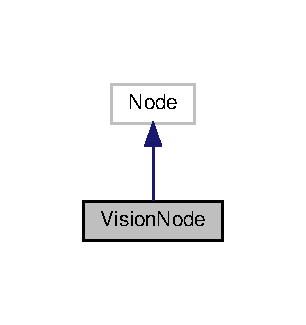
\includegraphics[width=147pt]{classVisionNode__inherit__graph}
\end{center}
\end{figure}


Collaboration diagram for Vision\+Node\+:
\nopagebreak
\begin{figure}[H]
\begin{center}
\leavevmode
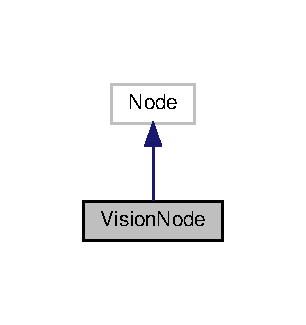
\includegraphics[width=147pt]{classVisionNode__coll__graph}
\end{center}
\end{figure}
\subsection*{Public Member Functions}
\begin{DoxyCompactItemize}
\item 
\mbox{\Hypertarget{classVisionNode_ab4d1d91b22f01874793337e9f3ae2083}\label{classVisionNode_ab4d1d91b22f01874793337e9f3ae2083}} 
void {\bfseries init\+Publisher} ()
\end{DoxyCompactItemize}
\subsection*{Private Member Functions}
\begin{DoxyCompactItemize}
\item 
\mbox{\Hypertarget{classVisionNode_aabbd33da50754623d30ba7c8c41dc2bc}\label{classVisionNode_aabbd33da50754623d30ba7c8c41dc2bc}} 
void {\bfseries raw\+Image\+Callback} (sensor\+\_\+msgs\+::msg\+::\+Image\+::\+Shared\+Ptr img\+\_\+msg)
\item 
\mbox{\Hypertarget{classVisionNode_ae2b6a2048ef69189b097ddc79b085603}\label{classVisionNode_ae2b6a2048ef69189b097ddc79b085603}} 
void {\bfseries pre\+Process\+Image} (cv\+::cuda\+::\+Gpu\+Mat \&gpu\+\_\+img)
\item 
\mbox{\Hypertarget{classVisionNode_a234d00d510249ff752af20a64b8618bd}\label{classVisionNode_a234d00d510249ff752af20a64b8618bd}} 
void {\bfseries apply\+Treshold} (cv\+::cuda\+::\+Gpu\+Mat \&gpu\+\_\+img, bool is\+\_\+white\+\_\+lane)
\item 
\mbox{\Hypertarget{classVisionNode_a6a6385ceaa4a9bb1e3d50dd2e55fb071}\label{classVisionNode_a6a6385ceaa4a9bb1e3d50dd2e55fb071}} 
void {\bfseries apply\+Morpho\+Transfo} (cv\+::cuda\+::\+Gpu\+Mat \&gpu\+\_\+img)
\item 
\mbox{\Hypertarget{classVisionNode_a7d60e45e5c445469ecb9f298c47bf5c8}\label{classVisionNode_a7d60e45e5c445469ecb9f298c47bf5c8}} 
void {\bfseries crop\+To\+R\+OI} (cv\+::cuda\+::\+Gpu\+Mat \&gpu\+\_\+img)
\item 
\mbox{\Hypertarget{classVisionNode_ace70a008db68efbf89cc43e485e06744}\label{classVisionNode_ace70a008db68efbf89cc43e485e06744}} 
void {\bfseries apply\+Canny\+Edge} (cv\+::cuda\+::\+Gpu\+Mat \&gpu\+\_\+img)
\item 
\mbox{\Hypertarget{classVisionNode_adf0f075a5d4706a887ba3198799a836f}\label{classVisionNode_adf0f075a5d4706a887ba3198799a836f}} 
std\+::vector$<$ cv\+::\+Vec4i $>$ {\bfseries get\+Lines} (cv\+::cuda\+::\+Gpu\+Mat \&gpu\+\_\+img)
\item 
\mbox{\Hypertarget{classVisionNode_a4d826b83d642f5033c796a8f89cd2b58}\label{classVisionNode_a4d826b83d642f5033c796a8f89cd2b58}} 
void {\bfseries publish\+Lane\+Positions} (std\+::vector$<$ cv\+::\+Vec4i $>$ \&lines, int img\+\_\+width, int img\+\_\+height)
\item 
\mbox{\Hypertarget{classVisionNode_afa493f144507b0de569a5935a54661f1}\label{classVisionNode_afa493f144507b0de569a5935a54661f1}} 
void {\bfseries publish\+Mask\+Img} (cv\+::cuda\+::\+Gpu\+Mat \&gpu\+\_\+img)
\item 
\mbox{\Hypertarget{classVisionNode_ac7f9f0b9c0c06f4446627de8d93dcd05}\label{classVisionNode_ac7f9f0b9c0c06f4446627de8d93dcd05}} 
void {\bfseries publish\+Edge\+Image} (cv\+::cuda\+::\+Gpu\+Mat \&gpu\+\_\+img)
\end{DoxyCompactItemize}
\subsection*{Private Attributes}
\begin{DoxyCompactItemize}
\item 
\mbox{\Hypertarget{classVisionNode_a7f2f6a8fc2898ec230d96a6df386f0ae}\label{classVisionNode_a7f2f6a8fc2898ec230d96a6df386f0ae}} 
rclcpp\+::\+Subscription$<$ sensor\+\_\+msgs\+::msg\+::\+Image $>$\+::Shared\+Ptr {\bfseries raw\+\_\+img\+\_\+sub\+\_\+}
\item 
\mbox{\Hypertarget{classVisionNode_aa4563584d251d6a0d2a3442a083ba8f0}\label{classVisionNode_aa4563584d251d6a0d2a3442a083ba8f0}} 
rclcpp\+::\+Publisher$<$ lane\+\_\+msgs\+::msg\+::\+Lane\+Positions $>$\+::Shared\+Ptr {\bfseries lane\+\_\+pos\+\_\+pub\+\_\+}
\item 
\mbox{\Hypertarget{classVisionNode_ab716281a28831e4e643d9ac14275a5d3}\label{classVisionNode_ab716281a28831e4e643d9ac14275a5d3}} 
image\+\_\+transport\+::\+Publisher {\bfseries edge\+\_\+img\+\_\+pub\+\_\+}
\item 
\mbox{\Hypertarget{classVisionNode_a6ab1e698ad581462c57aa056ac3fd245}\label{classVisionNode_a6ab1e698ad581462c57aa056ac3fd245}} 
image\+\_\+transport\+::\+Publisher {\bfseries mask\+\_\+pub\+\_\+}
\end{DoxyCompactItemize}


\subsection{Detailed Description}
Processes the image and extract lane positions. 

Apply treshold, gaussian blur, and canny edge to obtain only edges. Using a Hough transform, the lines following the edges are extracted and publish in a custom msg (Lane\+Positions) 

The documentation for this class was generated from the following files\+:\begin{DoxyCompactItemize}
\item 
lane\+\_\+keeping\+\_\+ws/src/classic\+\_\+vision/includes/Vision\+Node.\+hpp\item 
lane\+\_\+keeping\+\_\+ws/src/classic\+\_\+vision/src/Vision\+Node.\+cpp\end{DoxyCompactItemize}

%--- End generated contents ---

% Index
\backmatter
\newpage
\phantomsection
\clearemptydoublepage
\addcontentsline{toc}{chapter}{Index}
\printindex

\end{document}
